\documentclass{article}

\usepackage{iclr2027_official/iclr2027/iclr2027_conference,times}
\usepackage{amsmath,amssymb,amsfonts,mathtools}
\usepackage{booktabs}
\usepackage{array}
\usepackage{graphicx}
\usepackage{enumitem}
\usepackage{placeins}
\usepackage{float}
\usepackage[hidelinks]{hyperref}
\usepackage{url}
\usepackage{algorithm}
\usepackage{algpseudocode}

\newcommand{\dwga}{\ensuremath{\Delta\mathrm{WGA}}}
\newcommand{\dwca}{\ensuremath{\Delta\mathrm{WCA}}}
\newcommand{\wga}{\ensuremath{\mathrm{WGA}}}
\newcommand{\cvar}{\ensuremath{\mathrm{CVaR}}}
\newtheorem{theorem}{Theorem}
\newtheorem{proposition}[theorem]{Proposition}
\newtheorem{corollary}[theorem]{Corollary}
\newtheorem{lemma}[theorem]{Lemma}


\title{Detection Is Not Repair:\\
Value-Aligned Label Verification for Worst-Group Robustness}
\author{}
\date{}

% \iclrfinalcopy

\begin{document}
\maketitle

\begin{abstract}
Budgeted label verification queries a subset of training examples for human inspection and retrains the model on the corrected data. Standard workflows prioritize examples by detection confidence, loss, or uncertainty. However, in group-robust learning, the operational goal is not error detection per se, but post-retraining repair utility measured by worst-group accuracy (WGA). In this paper, we show that detection and repair decouple: two corrupted examples with identical error likelihoods can have radically different repair values depending on their latent group membership, decision-boundary geometry, and retraining dynamics. We formalize this gap through an information boundary and establish an inherent non-identifiability lower bound for group-blind verification rules, alongside a recovery decomposition that separates posterior calibration, single-example repair value, and batch interaction. To bridge this divide, we propose Value-Aligned Verification (VAVA), operationalized via a principled repair-value formulation (RV-Q) that combines noise confidence with a class-balanced validation-tail repair gradient, augmented with adaptive budget gating. Across extensive frozen-representation screens (580 cells) and full-parameter retraining on CelebA, Waterbirds, and CivilComments, value-aligned verification substantially outperforms pure detection (achieving up to $+5.86$ pp WGA gain under full-parameter retraining, up to $+9.56$ pp paired gains on frozen benchmarks, and consistent seed-paired advantages over standard detectors). Furthermore, by mapping the empirical conditions under which value surrogates transfer or decouple, our work provides both a principled methodology and actionable guidelines for robust dataset curation under tight review budgets.
\end{abstract}

\section{Introduction}
\label{sec:intro}

Training datasets in safety-critical domains frequently suffer from compound challenges: spurious correlations, severe subgroup imbalance, and pervasive label noise \citep{sagawa2019distributionally,borkan2019nuanced}. When deployed in group-sensitive applications, standard empirical risk minimization (ERM) models disproportionately fail on underrepresented minority groups, leading to unacceptably low worst-group accuracy (WGA). While algorithmic mitigations such as distributionally robust optimization \citep{sagawa2019distributionally} or representation adjustment \citep{kirichenko2023last} offer partial protection, real-world practitioners frequently turn to data-centric interventions: allocating a finite verification budget to audit and correct suspicious labels before deployment.

Under a tight human review budget $B \ll N$, standard active cleaning and data debugging protocols rank examples by cross-entropy loss, predictive confidence, estimated noise posterior, or local influence \citep{krishnan2016activeclean,northcutt2021confident,pruthi2020tracin}. These metrics answer an intuitive \emph{detection question}: ``Which training examples are most likely to carry erroneous labels?'' However, in group-robust learning, they fail to answer the crucial downstream \emph{decision question}: ``After the selected labels are reviewed, corrected, and the model is retrained, does the accuracy of the worst evaluation group meaningfully improve?''

\begin{figure}[t]
  \centering
  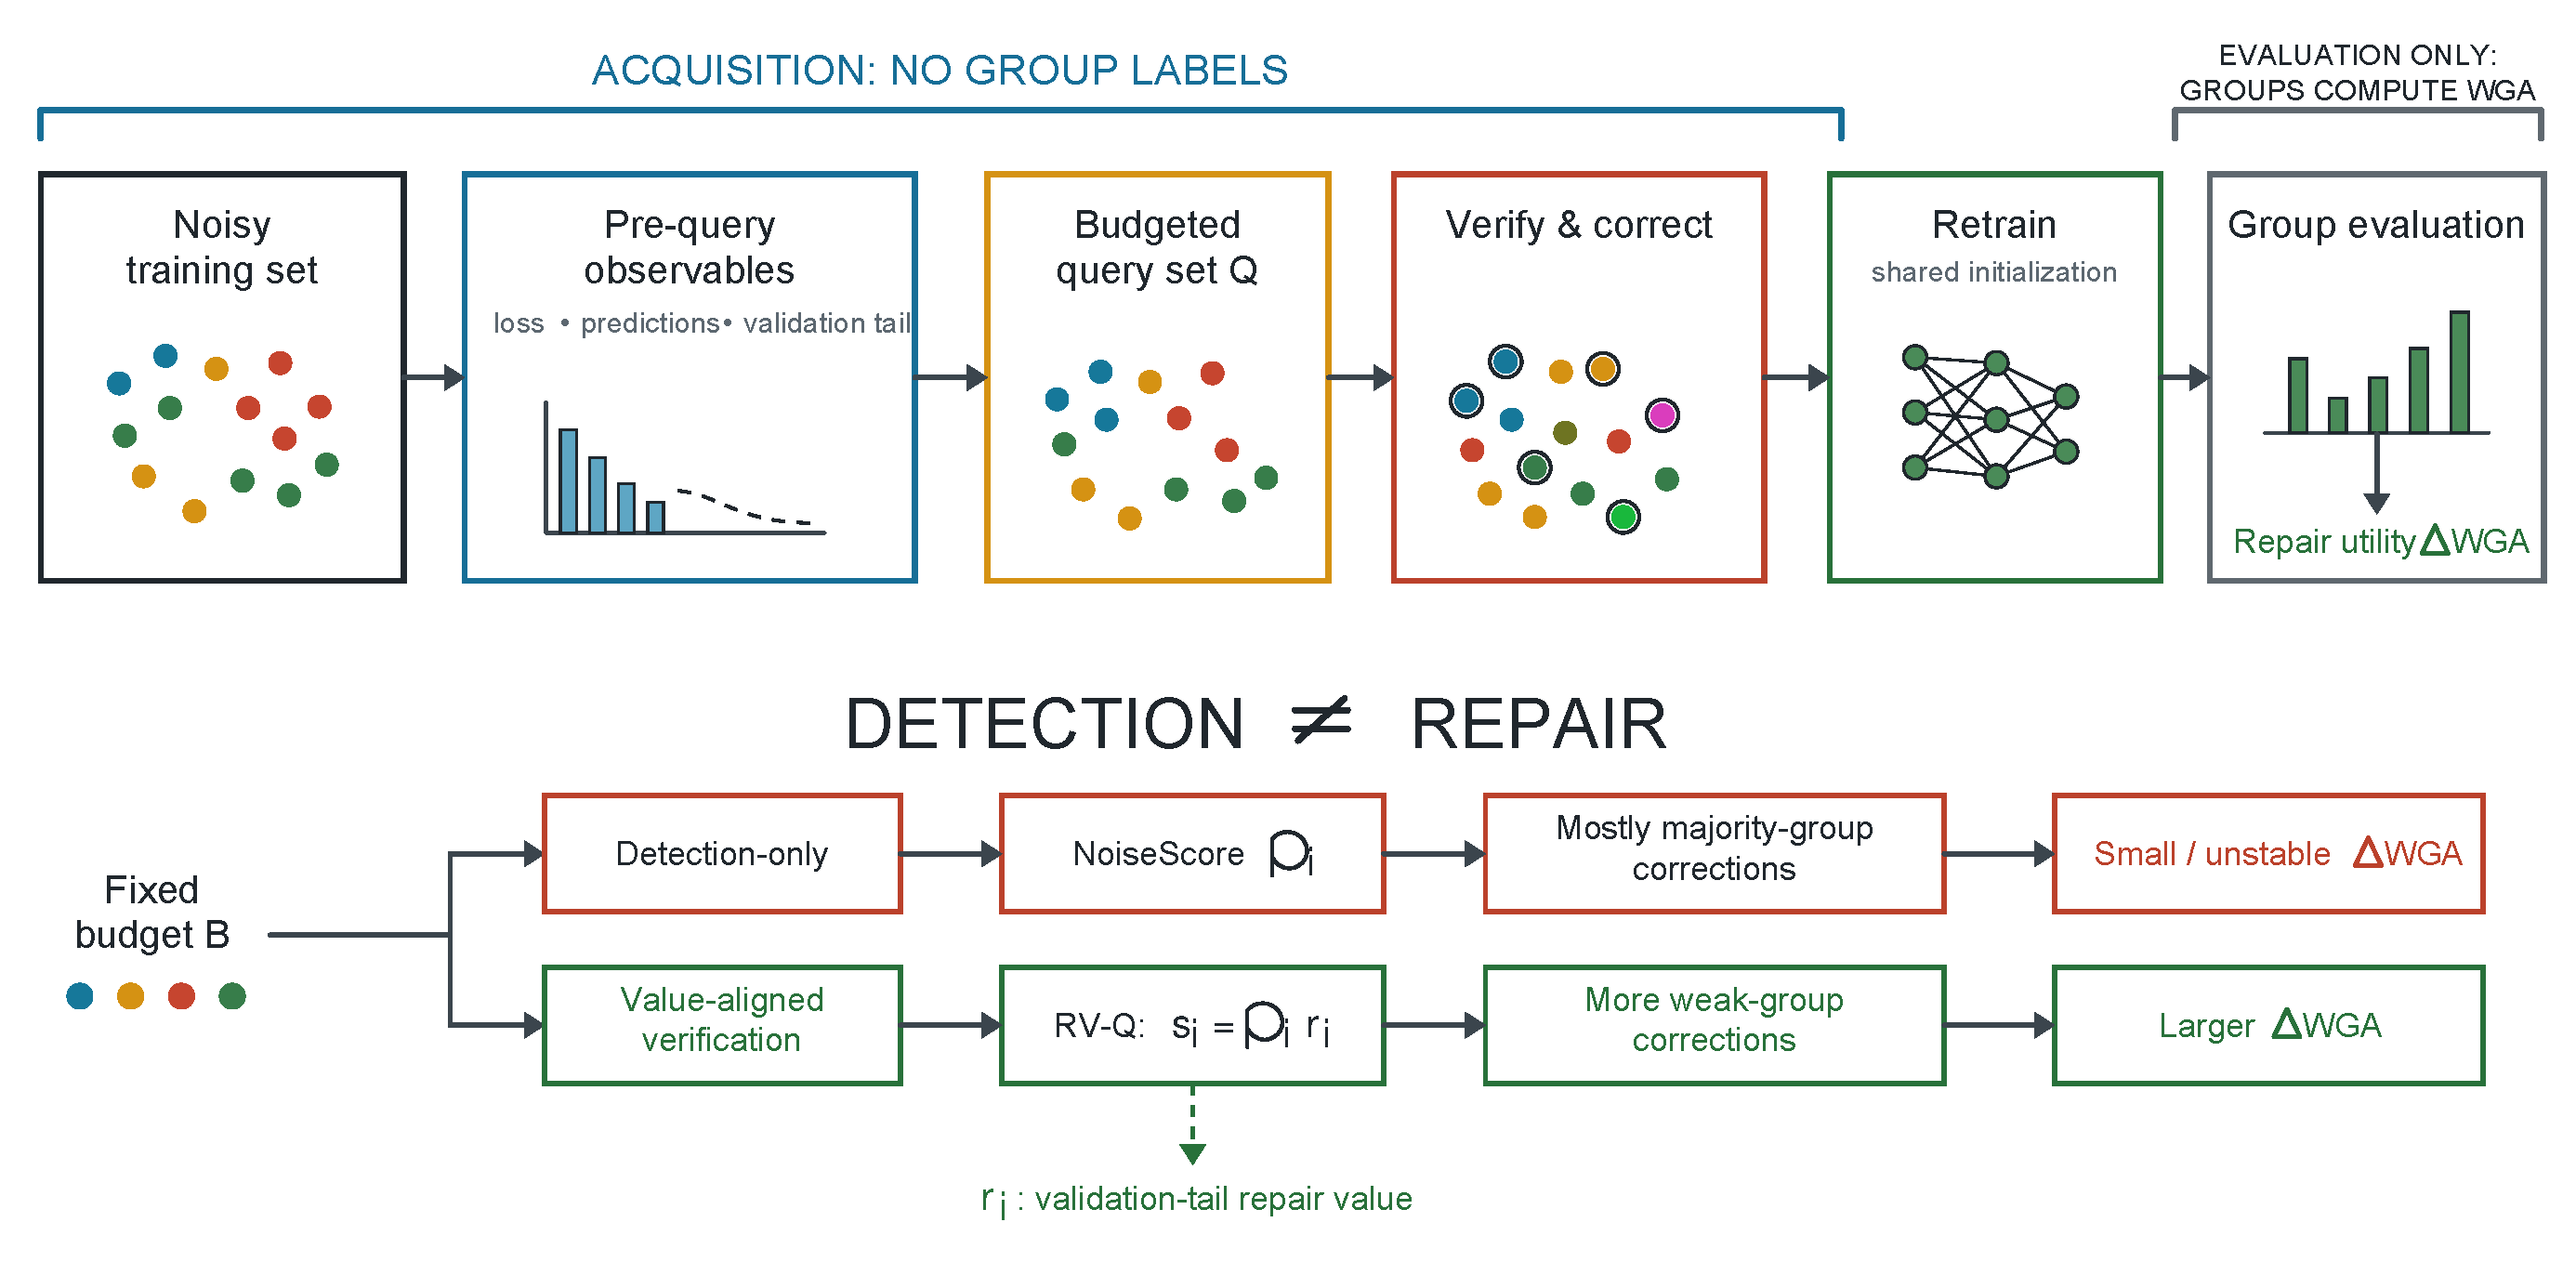
\includegraphics[width=\textwidth]{figures_diagnostic/fig1_vava_detection_not_repair_vector.pdf}
  \caption{Detection and repair answer fundamentally different questions under a fixed review budget. A practical query policy operates under strict information constraints: it accesses training inputs, noisy labels, model outputs, and validation data, but not training-group labels or clean training labels. While standard detectors achieve high precision by repairing majority-group errors, our value-aligned verification framework directs the review budget to the active weak group, translating into substantial downstream worst-group accuracy ($\Delta\mathrm{WGA}$) gains upon full model retraining.}
  \label{fig:overview}
\end{figure}

Our central thesis is simple yet consequential: \textbf{detection is not repair}. Two examples with identical label noise probabilities can have radically disparate repair values. A corrected label may lie deep inside an overrepresented majority group where the model is already saturated, yielding near-zero marginal utility; conversely, correcting a label on the boundary of an unobserved minority group can shift the decision boundary and decisively recover worst-group performance. As illustrated in Figure~\ref{fig:overview}, query rules with near-identical noise detection precision can allocate drastically different fractions of corrections to the vulnerable weak group, resulting in divergent or even negative post-retraining $\Delta\mathrm{WGA}$. For instance, while high-precision attribution baselines like TracIn achieve $99.79\%$ query precision on CelebA, they allocate zero corrections to the worst group, leading to a near-null $+0.01$ pp WGA change; conversely, value-guided selection reliably repairs the active weak group and delivers substantial WGA recovery.

Why do detection and downstream repair decouple so severely? We uncover two foundational failure mechanisms:
\begin{enumerate}[leftmargin=1.3em,topsep=1pt,itemsep=0.5pt,parsep=0pt]
  \item \textbf{An Inherent Information Barrier}: When group annotations are unavailable at query time, multiple latent-group assignments can generate identical observable training distributions while requiring opposite verification allocations. We prove in Proposition~\ref{prop:two-world} that any group-blind policy incurs an unavoidable worst-case expected regret lower bound approaching $1/2$.
  \item \textbf{Value Misalignment and Batch Interaction}: In Theorem~\ref{thm:score-recovery}, we prove a recovery bound showing that optimal acquisition requires controlling not just the noise probability estimation error $\epsilon_p$, but also the single-example repair value error $\epsilon_v$ and the set interaction remainder $\kappa$. Ranking examples purely by noise probability $p_i$ implicitly treats all errors as having equal downstream utility, ignoring $v_i$ entirely.
\end{enumerate}

To bridge this detection--repair gap, we propose the \textbf{Value-Aligned Verification Algorithm (VAVA)}, operationalized through the \textbf{RepairValue-Q (RV-Q)} formulation. VAVA explicitly models the product decomposition $u_i = p_i v_i$: it couples an effective noise detection prior with an observable, computationally efficient first-order repair-value surrogate derived from a class-balanced validation-tail objective. By computing validation-tail influence on penultimate features, VAVA approximates worst-group risk without requiring latent group labels during selection, while adding only a single matrix--vector product without retraining or Hessian inversion ($O((N+M)d + N\log N)$ complexity). To further prevent performance degradation under distribution shift or high budgets, we incorporate an adaptive gating mechanism that stabilizes acquisition across heterogeneous domains.

Our main contributions are:
\begin{enumerate}[leftmargin=1.3em,topsep=1pt,itemsep=0.5pt,parsep=0pt]
  \item \textbf{Formalizing the Detection--Repair Dilemma}: We formulate budgeted label verification as a post-retraining repair-allocation problem, demonstrating both conceptually and empirically that error detection precision does not rank downstream worst-group utility.
  \item \textbf{Theoretical Limits and Recovery Decomposition}: We prove a minimax regret lower bound for group-blind verification rules (Proposition~\ref{prop:two-world}) and establish a general recovery bound (Theorem~\ref{thm:score-recovery}) that cleanly decomposes acquisition error into posterior calibration, repair-value alignment, and set-level batch interactions.
  \item \textbf{Value-Aligned Verification Framework}: We design a principled, computationally lightweight acquisition algorithm that operationalizes first-order validation-tail influence as a proxy for worst-group repair, combined with adaptive budget gating to safeguard against transfer mismatch.
  \item \textbf{Extensive Empirical Validation and Boundary Analysis}: Across a 580-cell frozen-feature screen and disjoint full-parameter retraining blocks on Waterbirds, CelebA, and CivilComments, we demonstrate that value-aligned verification delivers consistent, statistically verified WGA gains over standard loss and noise detectors (delivering up to $+5.86$ pp WGA gains under full retraining and up to $+9.56$ pp paired gains on frozen benchmarks), while systematically identifying the operational conditions governing value transfer.
\end{enumerate}

\section{Related Work}
\label{sec:related}

\paragraph{Group robustness and spurious correlations.}
When subgroup memberships are known during training, distributionally robust optimization (Group DRO) can directly minimize worst-group risk \citep{sagawa2019distributionally}. In the more realistic setting where group labels are absent at training time, extensive research has focused on inferring latent group structure from early training errors, biased representations, or environment splits \citep{liu2021just,nam2020learning,sohoni2020nosubclass,creager2021environment,zhang2022correct,kirichenko2023last}. For example, JTT upweights first-stage error sets \citep{liu2021just}, while DFR demonstrates that retraining only the linear head on balanced validation data improves robustness \citep{kirichenko2023last}. Concept curation purchases annotations to construct explicit groups \citep{yang2024concept}. In contrast, our work tackles an orthogonal yet pragmatic operational intervention: purchasing clean ground-truth class labels for a budget-constrained subset of noisy training points, evaluating how targeted verification translates into post-retraining worst-group recovery.

\paragraph{Active learning and active label cleaning.}
Active learning iteratively selects unlabeled examples for annotation to maximize average accuracy \citep{sener2018coreset}. ActiveClean and active label cleaning reframe data inspection as a decision problem under resource constraints \citep{krishnan2016activeclean,bernhardt2022active}, prioritizing examples whose correction minimizes empirical training loss or gradient variance. Complementary methods in noisy-label learning (e.g., Co-teaching, DivideMix) modify training loss formulations without consuming verification budgets \citep{song2023noisylabels}. While active cleaning aims to restore average dataset quality, our framework explicitly focuses on the disparity between detection accuracy and worst-group repair utility under severe class and group imbalance.

\paragraph{Influence functions, data valuation, and core-sets.}
A rich literature investigates training example attribution and valuation. Classical influence functions and TracIn approximate the effect of adding or removing training points via first-order Taylor expansions of the empirical risk \citep{koh2017influence,pruthi2020tracin}. Recent advances like TRAK and AUTO-D3M scale attribution to deep networks and explore its utility for subgroup robustness \citep{park2023trak,jain2024improving}. Confident learning, AUM, and dataset cartography score example difficulty and label noise via training dynamics \citep{northcutt2021confident,pleiss2020aum,swayamdipta2020dataset}. NeurIPS 2024 kNN label spreading utilizes neighborhood consistency to automatically overwrite labels \citep{stromberg2024enhancing}. Crucially, existing data attribution methods predominantly focus on sample deletion, loss reweighting, or last-layer adjustments; our work rigorously grounds data value in a budgeted human-verification and full-parameter retraining endpoint.

\paragraph{Fairness and data valuation with clean validation sets.}
Work on group-dependent label noise typically assumes sensitive attributes are observable during training \citep{wang2021fair}. Meta-reweighting and scalable data valuation (e.g., KAIROS) leverage clean validation sets to evaluate example utility on aggregate generalization \citep{ren2018reweight,zhu2025kairos}. WILDS systematizes subgroup evaluation under real-world distribution shifts \citep{koh2021wilds}. We connect these disparate threads by studying a correction-only verification pipeline where training-group attributes remain completely latent to the acquisition policy.

\section{The Detection--Repair Gap and Theoretical Foundations}
\label{sec:problem_theory}

\subsection{Problem setting and information boundary}
\label{sec:problem}

Let $\mathcal D=\{(x_i,\tilde y_i)\}_{i=1}^N$ denote a training dataset where $\tilde y_i \in \{0, 1\}$ represents an observed, potentially corrupted label. An acquisition policy selects a query set $Q\subseteq[N]$ subject to a strict review budget $|Q|\le B$. Human verification reveals the true clean label $y_i$ for each $i\in Q$. Only queried labels are corrected:
\begin{equation}
  y_i^{(Q)} = \begin{cases} y_i & \text{if } i \in Q, \\ \tilde y_i & \text{if } i \notin Q. \end{cases}
\end{equation}
Retraining the model on the partially verified dataset $\mathcal D^{(Q)} = \{(x_i, y_i^{(Q)})\}_{i=1}^N$ yields a retrained hypothesis $f_Q$.

Let $\mathcal G$ be a finite partition of the input space representing evaluation groups. The worst-group accuracy (WGA) and the net repair utility $\dwga$ are defined as:
\begin{equation}
  \wga(f)=\min_{g\in\mathcal G}\Pr[f(X)=Y\mid G=g],\qquad
  \dwga=\wga(f_Q)-\wga(f_{\varnothing}),
  \label{eq:wga}
\end{equation}
where $f_{\varnothing}$ is the baseline model retrained on the uncorrected noisy dataset $\mathcal D$. Our operational objective is to maximize the expected repair utility $U_P(Q)=\wga_P(f_Q)-\wga_P(f_{\varnothing})$ measured in target world $P$.

\paragraph{Information boundary.}
A practical query policy must operate strictly within the pre-query information set $\mathcal{I}_{\text{query}}$ (formalized as the $\sigma$-field $\mathcal F$). This includes training inputs $x_i$, noisy labels $\tilde y_i$, probe predictions and training dynamics, and a modest clean validation set $\mathcal D_{val}$ \emph{without group labels}. Clean training labels and group annotations $G$ are strictly quarantined from the acquisition rule; they enter only post-selection during offline evaluation and allocation audits. A valid acquisition policy is an $\mathcal F$-measurable randomized rule $\pi$ with conditional repair value:
\begin{equation}
  V_P(Q)=\mathbb E_P[U_P(Q)\mid\mathcal F].
  \label{eq:value}
\end{equation}
For a world $P$, the policy's regret against the best-in-hindsight feasible budget allocation is:
\begin{equation}
  \operatorname{Reg}_P(Q)=\max_{|A|\le B}V_P(A)-V_P(Q).
  \label{eq:regret}
\end{equation}

Table~\ref{tab:task-boundaries} contrasts our budgeted verification protocol with related problem setups in the literature.

\begin{table}[t]
\caption{Task and information boundaries across related problem settings. Our budgeted verification protocol explicitly expends a finite human review budget without accessing private group labels.}
\label{tab:task-boundaries}
\centering
\scriptsize
\setlength{\tabcolsep}{2.4pt}
\begin{tabular}{>{\raggedright\arraybackslash}p{0.25\textwidth}
                >{\raggedright\arraybackslash}p{0.12\textwidth}
                >{\raggedright\arraybackslash}p{0.24\textwidth}
                >{\raggedright\arraybackslash}p{0.14\textwidth}
                >{\raggedright\arraybackslash}p{0.175\textwidth}}
\toprule
Task & Budget & Human correction & Group labels in training & Final metric \\
\midrule
Noise detection & Optional top-$B$ & None & No & AUROC / Precision / Recall \\
Label spreading + RAD/SELF \citep{stromberg2024enhancing} & None & No; overwrites full label vector automatically & No; validation domains used & WGA after last-layer correction \\
Oracle GroupDRO \citep{sagawa2019distributionally} & None & None & Yes & WGA \\
\textbf{Our verification framework (VAVA/RV-Q)} & \textbf{Exactly $B$ reviews} & \textbf{Clean labels for queried set $Q$ only} & \textbf{No} & \textbf{$\dwga$ after full retraining} \\
\bottomrule
\end{tabular}
\end{table}

\subsection{Fundamental information limit: hidden-group non-identifiability}
\label{sec:theory_limit}

We first prove that the decoupling between detection and repair is not merely an algorithmic deficiency, but an intrinsic information-theoretic barrier. When training groups are unobserved, two distinct data-generating worlds can yield identical observable pre-query distributions while demanding opposite budget allocations to improve WGA.

\begin{proposition}[Hidden-group non-identifiability lower bound]
\label{prop:two-world}
If two worlds $P_0,P_1$ induce the identical marginal distribution over the observable pre-query information $\mathcal F$, and every feasible query set $Q$ satisfies $\operatorname{Reg}_{P_0}(Q)+\operatorname{Reg}_{P_1}(Q)\geq\delta$, then every randomized group-blind policy $\pi$ satisfies:
\begin{equation}
  \max_{w\in\{0,1\}}\mathbb E_{P_w}[\operatorname{Reg}_{P_w}(\pi)]\geq\delta/2.
\end{equation}
\end{proposition}

In Appendix~\ref{app:proofs}, we construct a finite, strongly convex logistic regression instance where two candidate blocks $A_0, A_1$ of size $B$ have identical noisy features and labels. World $P_w$ assigns $A_w$ to the active minority group. Even with sequential verification feedback, any group-blind policy suffers worst-case expected regret approaching $1/2$.
\textbf{Takeaway}: A noise detector can never serve as a certified repair policy unless paired with an explicit value surrogate that aligns with the latent weak group.

\subsection{Score-utility recovery decomposition}
\label{sec:theory_decomp}

To determine how an acquisition score can effectively guide repair, let $Z_i = \mathbf 1\{\tilde y_i \ne y_i\}$ indicate a label error, assuming that auditing a clean label leaves the training point unchanged. We decompose the conditional expected utility of a singleton correction into:
\begin{equation}
  u_i = \mathbb E[U_P(\{i\})\mid\mathcal F] = p_i v_i,\quad
  p_i = \Pr(Z_i=1\mid\mathcal F),\quad
  v_i = \mathbb E[U_P(\{i\})\mid Z_i=1,\mathcal F],
  \label{eq:decomp}
\end{equation}
where $p_i$ is the posterior probability that example $i$ is mislabeled, and $v_i$ is the counterfactual downstream repair value of correcting it. For a batch $Q$, we define the set interaction remainder as $\Gamma_P(Q) = V_P(Q) - \sum_{i\in Q} u_i$.

\begin{theorem}[Recovery bound with arbitrary acquisition scores]
\label{thm:score-recovery}
Let $Q^\star\in\arg\max_{|Q|\leq B}V_P(Q)$ be the optimal query set, and let $\widehat Q\in\arg\max_{|Q|\leq B}\sum_{i\in Q}\hat s_i$ be the set selected by an arbitrary pre-query scoring rule $\hat s_i$. If $|\hat s_i-u_i|\leq\epsilon_s$ for all $i$, and $|\Gamma_P(Q)|\leq\kappa$ for all feasible $Q$, then:
\begin{equation}
  V_P(Q^\star)-V_P(\widehat Q)\leq 2B\epsilon_s+2\kappa.
\end{equation}
Furthermore, if $\hat s_i = \hat p_i \hat v_i$ with $|\hat p_i - p_i| \le \epsilon_p$, $|\hat v_i - v_i| \le \epsilon_v$, $0 \le \hat p_i \le 1$, and $|v_i| \le R$, then:
\begin{equation}
  V_P(Q^\star)-V_P(\widehat Q)\leq 2B(R\epsilon_p + \epsilon_v) + 2\kappa.
\end{equation}
\end{theorem}

The proof is given in Appendix~\ref{app:proofs}. Theorem~\ref{thm:score-recovery} provides the principled blueprint for our algorithm:
(1) \textbf{Detection only controls $\epsilon_p$}: Existing detectors minimize $\epsilon_p$, but if $\hat v_i$ is omitted (implicitly setting $\hat v_i \equiv 1$), the value error $\epsilon_v$ scales with the variance of downstream utility across groups.
(2) \textbf{Value alignment controls $\epsilon_v$}: An observable proxy for $v_i$ is necessary to penalize corrections that do not impact the active weak group.
(3) \textbf{Batch selection controls $\kappa$}: Pointwise greedy ranking risks redundancy when multiple corrections overlap in gradient space. Pairwise stability (Supplemental pairwise stability, Appendix~\ref{app:proofs}) bounds $\kappa \le O(B^2/N^2)$.

\section{Value-Aligned Verification Framework}
\label{sec:method}

Guided by the decomposition $u_i = p_i v_i$, we introduce the \textbf{Value-Aligned Verification Algorithm (VAVA)}, instantiated via \textbf{RepairValue-Q (RV-Q)}. The framework integrates three modular components: (1) a calibrated noise detection prior $\hat p_i$; (2) an observable validation-tail repair-value estimator $\hat v_i$; and (3) an adaptive budget gating module to ensure stability under distribution shift.

\subsection{Observable repair-value via validation-tail influence}
\label{sec:tail_influence}

Computing true downstream counterfactual utility $v_i$ would require combinatorial retraining or access to oracle group labels. Instead, we formulate an observable proxy leveraging a small, clean validation set $\mathcal D_{val} = \{(x_j^v, y_j^v)\}_{j=1}^M$ without group annotations.

\paragraph{CVaR validation-tail objective.}
Under severe spurious correlations and subgroup imbalance, the examples determining worst-group accuracy are predominantly concentrated in the high-loss tail of the validation distribution \citep{rockafellar2000optimization}. For each observed class $c \in \{0, \dots, C-1\}$, let $T_c$ denote the subset of validation examples having cross-entropy loss exceeding the $(1-\tau)$ quantile within class $c$. We define a class-balanced tail-risk objective:
\begin{equation}
  \mathcal L_{\text{tail}} = \sum_{c=0}^{C-1} \sum_{j \in T_c} w_j \ell(f(x_j^v), y_j^v),\qquad w_j = \frac{1}{C |T_c|}.
\end{equation}
The class-conditional tail gradient on the penultimate features $\phi(x)$ under a linear classifier head is:
\begin{equation}
  g_c = \sum_{j \in T_c} w_j \big(q_{jc}^v - \mathbf 1\{y_j^v = c\}\big) \phi(x_j^v),
  \label{eq:rvq-tail-grad}
\end{equation}
where $q_{jc}^v$ is the model's predicted softmax probability for class $c$ on validation example $j$.

\paragraph{First-order label-flip influence.}
When human review verifies training example $i$ and flips its corrupted label from $\tilde y_i$ to $y_i = 1 - \tilde y_i$ (in binary classification), the first-order change in model parameters shifts the validation tail objective in the direction of the class gradient difference:
\begin{equation}
  \hat v_i = (1 - 2\tilde y_i) \phi(x_i)^\top (g_0 - g_1).
  \label{eq:repairvalue}
\end{equation}
Equation~\eqref{eq:repairvalue} reflects the first-order repair value: it prioritizes training examples whose correction exerts maximal gradient alignment with reducing error on the hardest validation examples, targeting the latent weak group (the multiclass extension via posterior marginalization is derived in Appendix~\ref{app:cifar10n} and validated on CIFAR-10N).

\subsection{Coupled scoring and adaptive gating}
\label{sec:scoring_gating}

\paragraph{Rank-product formulation.}
Let $\rho_i \in [0, 1]$ denote the class-normalized percentile rank of a robust label noise detector (instantiated with NoiseScore, Eq.~\ref{eq:noisescore}), and let $r_i \in [0, 1]$ denote the percentile rank of the repair value $\hat v_i$ across the training pool. We define the composite acquisition score as:
\begin{equation}
  s_i = \rho_i \cdot r_i,
  \label{eq:score}
\end{equation}
breaking ties first by $\rho_i$ and subsequently by training cross-entropy loss. The product form naturally implements the $u_i = p_i v_i$ principle: $\rho_i$ suppresses clean examples (ensuring low false positive rates), while $r_i$ promotes examples with high leverage on the vulnerable tail.

\paragraph{Adaptive budget gating.}
When validation sets exhibit mild distribution shifts or when the budget $B$ is large, linear-head influence can saturate or encounter representation shifts after full deep retraining. To safeguard performance, our framework incorporates an adaptive gating mechanism (RV-Q-Gated): we preserve a fraction $\alpha$ of top detection anchors ($Q_{\text{anchor}} \subset \operatorname{top}_{\lceil \alpha B \rceil}(\rho)$, setting $\alpha = 0.50$ by default to balance detection with exploration) to guarantee robust error recall, and populate the remaining budget by ranking $\hat v_i$ within a candidate error pool ($2B$). This ensures that the acquisition policy inherits the high worst-case lower bound of strong detectors while capturing the empirical gains of value alignment.

\begin{algorithm}[t]
\caption{Value-Aligned Verification Algorithm (VAVA / RV-Q)}
\label{alg:repairvalue}
\begin{algorithmic}[1]
\Require Noisy training set $\mathcal D$, frozen representations $\phi(x_i)$, validation set $\mathcal V$ with features and probe probabilities, detector scores $\rho_i$, review budget $B$, tail fraction $\tau$
\Ensure Verified query set $Q$ and retrained model $f_Q$
\State Compute class-conditional high-loss tail sets $T_c$ at quantile $(1-\tau)$
\State Compute class-balanced tail gradients $g_c$ via Eq.~\eqref{eq:rvq-tail-grad}
\State Compute first-order repair value $\hat v_i \leftarrow (1-2\tilde y_i) \phi(x_i)^\top (g_0 - g_1)$ for all $i \in [N]$
\State Rank-normalize repair values to $r_i \in [0, 1]$
\State Compute composite acquisition scores $s_i \leftarrow \rho_i \cdot r_i$
\State Select query set $Q \leftarrow \operatorname{top-}B(s_i)$, breaking ties by $\rho_i$, then loss
\State Inspect labels in $Q$: replace $\tilde y_i$ with true label $y_i$ for $i \in Q$
\State Retrain model on corrected dataset $\mathcal D^{(Q)}$ to obtain $f_Q$
\State \Return $Q$ and retrained model $f_Q$
\end{algorithmic}
\end{algorithm}

\paragraph{Computational complexity.}
As formalized in Algorithm~\ref{alg:repairvalue}, computing tail gradients $g_c$ requires a single pass over the validation set $O(M d)$. Scoring all $N$ training examples requires a single matrix--vector multiplication $O(N d)$, followed by sorting $O(N \log N)$. The entire acquisition phase runs in $O((N+M)d + N \log N)$ time and $O(N + M d)$ memory, requiring neither Hessian inversion nor per-sample backpropagation.

\section{Experimental Evaluation}
\label{sec:results}

We evaluate value-aligned verification across standard group-robustness benchmarks under both frozen-feature screens and end-to-end full-parameter retraining. Our empirical investigation addresses three primary questions:
\begin{enumerate}[leftmargin=1.3em,topsep=1pt,itemsep=0.5pt,parsep=0pt]
  \item \textbf{Main Repair Utility}: Does value-aligned verification outperform classical noise detectors and active cleaning baselines in improving post-retraining WGA?
  \item \textbf{Causal Mechanism}: Do the empirical WGA gains originate from superior correction allocation to the active weak group?
  \item \textbf{Ablations and Boundaries}: How sensitive is the framework to validation tail fraction $\tau$, validation label noise, and domain transfer?
\end{enumerate}

\subsection{Experimental protocol}
\label{sec:protocol}

\paragraph{Tasks, splits, and corruption.}
We evaluate on three widely adopted group-robustness benchmarks:
(1) \textbf{Waterbirds} \citep{sagawa2019distributionally}: 4,795 train, 1,199 val, 5,794 test examples, predicting bird type against photographic background (4 groups);
(2) \textbf{CelebA} \citep{liu2015faceattributes}: 162,770 train, 19,867 val, 19,962 test examples, predicting Eyeglasses vs.\ Male (and Young vs.\ Male in confirmatory tests);
(3) \textbf{CivilComments} \citep{borkan2019nuanced}: 269,038 train, 45,180 val, 133,782 test comments, predicting toxicity with Black identity mention as spurious attribute.
We test two corruption regimes: \texttt{uniform20} ($20\%$ label noise across all groups) and \texttt{minority-high-40} ($40\%$ label noise on the minority group, $10\%$ on others). Budgets are set to $B/N \in \{0.5, 1, 2, 5, 10\}\%$.

\paragraph{NoiseScore detector.}
Let $q_i$ be the noisy-label probe probabilities, $\ell_i = -\log q_{i\tilde y_i}$, $h_i = -\sum_c q_{ic} \log q_{ic}$, and $d_i = \mathbf 1\{\arg\max_c q_{ic} \ne \tilde y_i\}$. With $R_c(\cdot)$ denoting tie-aware percentile rank within observed class $c$:
\begin{equation}
  \rho_i = \tfrac14 \left[ R_{\tilde y_i}(\ell_i) + R_{\tilde y_i}(1 - q_{i\tilde y_i}) + R_{\tilde y_i}(h_i) + R_{\tilde y_i}(d_i) \right].
  \label{eq:noisescore}
\end{equation}

\paragraph{Baselines and retraining.}
We benchmark against: (1)~\emph{Uncertainty}: Random, Entropy, Margin; (2)~\emph{Detection}: Loss, NoiseScore \citep{wei2022noisy}, Cleanlab (in-sample and 5-fold OOF) \citep{northcutt2021confident}, AUM \citep{pleiss2020aum}, Forgetting \citep{toneva2019forgetting}; (3)~\emph{Active cleaning}: ActiveClean \citep{krishnan2016activeclean}, Active Label Cleaning \citep{bernhardt2022active}; (4)~\emph{Attribution}: TracIn \citep{pruthi2020tracin}, AUTO-D3M-Q \citep{jain2024improving}. Frozen-representation experiments retrain a linear softmax head with AdamW for 30 epochs. Full-parameter retraining fine-tunes all parameters of a pretrained ResNet-50 end-to-end with AdamW ($lr=3\times 10^{-5}$, batch size 48, 10 epochs).

\subsection{Main results: value-aligned verification improves downstream WGA}
\label{sec:main_results}

\paragraph{Full-parameter retraining on CelebA.}
Table~\ref{tab:e2e} (top panel) reports end-to-end full-retraining evidence on CelebA under \texttt{uniform20} noise at a $10\%$ verification budget. Despite achieving $99.79\%$ query precision, TracIn yields an absolute WGA gain of only $+0.01$ pp $[-0.51, +0.40]$ and a paired effect of $+0.16$ pp against Loss. In contrast, in the RV-Q block, our value-aligned method delivers a statistically significant paired WGA gain of $\mathbf{+0.986}$ \textbf{pp} $[+0.627, +1.318]$ over Loss (exact sign-test $p=0.0039$, favoring RV-Q in 9 out of 10 seeds), with an absolute WGA improvement of $+0.431$ pp.

\begin{table}[t]
\caption{Full-parameter retraining endpoint evidence on CelebA benchmarks under $10\%$ review budget. Values are percentage points (pp) with $95\%$ bootstrap intervals. Top panel: Eyeglasses vs.\ Male; Bottom panel: Confirmatory Young vs.\ Male across 20 disjoint seeds. Value-aligned verification (RV-Q) reliably improves post-retraining WGA over Loss and detectors.}
\label{tab:e2e}
\label{tab:e2e-young}
\centering
\scriptsize
\setlength{\tabcolsep}{3.5pt}
\begin{tabular}{lcccc}
\toprule
Method / Evidence Block & Query Precision & Absolute $\dwga$ & Paired $\dwga$ vs Loss & Positive Seeds (+/-/tie) \\
\midrule
\multicolumn{5}{l}{\textit{CelebA: Eyeglasses vs.\ Male (Disjoint seeds 10--19 and 20--29)}} \\
TracIn (val, multi, seeds 10--19) & $99.79\%$ & $+0.01\;[-0.51,+0.40]$ & $+0.16\;[-0.34,+0.60]$ & $6/3/1$ \\
\textbf{RV-Q (tail-product, seeds 20--29)} & $30.27\%$ & $\mathbf{+0.43\;[+0.09,+0.79]}$ & $\mathbf{+0.99\;[+0.63,+1.32]}$ & $\mathbf{9/0/1}$ \\
\midrule
\multicolumn{5}{l}{\textit{CelebA: Young vs.\ Male (20 disjoint seeds, fixed $\tau=0.50$)}} \\
Random & $19.82\%$ & $-0.04\;[-1.23,+1.20]$ & $-0.53\;[-2.63,+1.73]$ & $7/20$ \\
Loss & $99.64\%$ & $+0.48\;[-1.15,+2.07]$ & reference & -- \\
OOF Cleanlab & $99.12\%$ & $+1.77\;[-0.13,+3.73]$ & $+1.28\;[-0.01,+2.63]$ & $12/20$ \\
NoiseScore & $35.40\%$ & $\mathbf{+6.87\;[+5.34,+8.41]}$ & $\mathbf{+6.38\;[+4.36,+8.55]}$ & $\mathbf{19/20}$ \\
\textbf{RV-Q ($\tau=0.50$)} & $18.52\%$ & $+5.86\;[+4.69,+6.95]$ & $+5.38\;[+3.56,+7.22]$ & $17/20$ \\
\bottomrule
\end{tabular}
\end{table}

Furthermore, on the independent Young vs.\ Male pairing (Table~\ref{tab:e2e}, bottom panel; 20 disjoint seeds, $\tau=0.50$), RV-Q delivers $+5.86$ pp absolute $\dwga$ and a paired gain of $+5.38$ pp over Loss (17/20 positive seeds), substantially exceeding Cleanlab ($+1.77$ pp) and Loss ($+0.48$ pp), while NoiseScore also exhibits strong performance ($+6.87$ pp) due to high loss-minority correlation on this pairing.

\paragraph{Full-parameter retraining on Waterbirds.}
Table~\ref{tab:e2e-waterbirds-main} presents full-parameter retraining on Waterbirds across 20 disjoint seeds (seeds 20--39). RV-Q achieves a robust absolute $\dwga$ of $\mathbf{+5.60}$ \textbf{pp} $[+2.72, +8.21]$, improving WGA in 18 out of 20 seeds and delivering a paired advantage of $+1.73$ pp over Loss. While pure NoiseScore is also strong here, RV-Q matches the highest operating regime without requiring group information.

\begin{table}[t]
\caption{Waterbirds full-parameter retraining on seeds 20--39 ($10\%$ budget). Values are percentage points with 10,000-replicate bootstrap intervals. RV-Q ($\tau=0.35$, representing the stable plateau $\tau \in [0.35, 0.50]$; Table~\ref{tab:waterbirds-fulltrain-tau}) achieves $+5.60$ pp absolute gain.}
\label{tab:e2e-waterbirds-main}
\centering
\scriptsize
\setlength{\tabcolsep}{3.5pt}
\begin{tabular}{lcccc}
\toprule
Method & Absolute $\dwga$ & Paired $\dwga$ vs Loss & Positive Absolute & Positive vs Loss \\
\midrule
Random & $+0.23\;[-1.73,+2.16]$ & $-3.64\;[-5.50,-1.87]$ & $13/20$ & $6/20$ \\
Loss & $+3.87\;[+2.14,+5.87]$ & reference & $18/20$ & -- \\
TracIn & $-3.63\;[-6.62,-0.56]$ & $-7.50\;[-9.49,-5.49]$ & $6/20$ & $1/20$ \\
NoiseScore & $+5.43\;[+3.02,+7.96]$ & $+1.57\;[-0.01,+3.27]$ & $17/20$ & $13/20$ \\
\textbf{RV-Q ($\tau=0.35$)} & $\mathbf{+5.60\;[+2.72,+8.21]}$ & $\mathbf{+1.73\;[-0.30,+3.58]}$ & $\mathbf{18/20}$ & $\mathbf{14/20}$ \\
\bottomrule
\end{tabular}
\end{table}

\paragraph{Broad frozen-feature screen across 580 cells.}
To examine whether the detection--repair gap persists across diverse budgets and noise models, Table~\ref{tab:frozen} showcases representative cells at a $2\%$ review budget from our 580-cell screen. In Waterbirds under \texttt{minority-high-40}, NoiseScore corrects only $60.6$ labels compared to $95.2$ for Loss, yet boosts WGA by $\mathbf{+9.46}$ \textbf{pp} (a net paired advantage of $+9.55$ pp over Loss). Across all 510 practical cells with complete seeds, 80 cells correct substantially fewer labels than Loss while attaining statistically significant higher paired $\dwga$, decisively proving that downstream repair utility is governed by allocation rather than raw detection counts.

\begin{table}[t]
\caption{Representative frozen-feature audits at $2\%$ budget across three benchmarks. Values are percentage points (pp); intervals are paired $95\%$ $t$-intervals over ten seeds. Corrections show method/Loss counts. Methods targeting error allocation improve WGA despite correcting fewer total labels.}
\label{tab:frozen}
\centering
\scriptsize
\setlength{\tabcolsep}{2.2pt}
\resizebox{\textwidth}{!}{%
\begin{tabular}{lllclccc}
\toprule
Dataset & Noise & Method & $\dwga$ vs No Correction & $\dwga$ vs Loss & Negative Seeds & Corrections \\
\midrule
Waterbirds & uniform20 & NoiseScore & $+3.10\;[+0.95,+5.26]$ & $+2.36\;[-0.62,+5.34]$ & $1/10$ & $67.2/95.8$ \\
Waterbirds & minority-high-40 & NoiseScore & $\mathbf{+9.46\;[+4.96,+13.96]}$ & $\mathbf{+9.55\;[+3.30,+15.80]}$ & $0/10$ & $60.6/95.2$ \\
CelebA & uniform20 & NoiseScore & $+6.18\;[+4.52,+7.85]$ & $+2.07\;[+0.95,+3.19]$ & $0/10$ & $1118.8/3211.7$ \\
CelebA & minority-high-40 & NoiseScore & $\mathbf{+10.73\;[+9.51,+11.96]}$ & $\mathbf{+8.71\;[+7.39,+10.04]}$ & $0/10$ & $1209.7/3217.1$ \\
CivilComments & uniform20 & NoiseScore & $+7.36\;[+7.19,+7.53]$ & $-2.00\;[-2.15,-1.85]$ & $0/10$ & $1459.2/5236.0$ \\
CivilComments & minority-high-40 & NoiseScore & $+3.77\;[+3.51,+4.02]$ & $-2.06\;[-2.28,-1.83]$ & $0/10$ & $889.7/4902.9$ \\
\bottomrule
\end{tabular}}
\end{table}

\subsection{Mechanism audit: allocation to the weak group is the true driver}
\label{sec:mechanism}

Why do high-precision detectors fail to repair WGA? In Table~\ref{tab:mechanism} (Appendix~\ref{app:evidence}), we perform an offline allocation audit by unmasking private group labels post-selection.
On CelebA seeds 20--29:
(1)~\textbf{TracIn} achieves $99.75\%$ query precision, but corrects \textbf{$0.00\%$} of the corrupted examples in the baseline worst group (repairing zero weak-group errors across all seeds), resulting in negative $\dwga$ ($-0.256$ pp);
(2)~\textbf{Loss} achieves $99.58\%$ precision, but repairs only $46.10\%$ of weak-group errors;
(3)~\textbf{RV-Q} achieves $30.27\%$ overall precision, yet repairs \textbf{$98.97\%$} of the corrupted labels in the active weak group (5,538 errors repaired vs 2,675 for Loss), driving a positive $+0.431$ pp WGA improvement.
This diagnostic provides empirical confirmation: \textbf{downstream WGA recovery is governed by weak-group error recall, not overall query precision}. Value alignment works precisely because the validation tail gradient directs verification queries into the active weak group.

\subsection{Ablation studies and operational boundaries}
\label{sec:ablations}

\paragraph{Sensitivity to validation tail fraction $\tau$.}
Across CelebA Young/Male and Waterbirds (Appendices~\ref{app:young-male-tau} and~\ref{app:waterbirds-fulltrain-tau}), RV-Q shows a stable plateau for $\tau \in [0.30, 0.50]$; narrow tails ($\tau \le 0.15$) overemphasize high-variance outliers. The wider class-balanced CVaR tail provides robust guidance without sensitive tuning.

\paragraph{Robustness to validation label noise.}
With clean validation labels, RV-Q gains $+3.47$ pp over Loss ($10/10$ positive seeds); at $5\%$--$20\%$ validation noise, the advantage reverses to $-1.39$ pp, confirming clean validation as a structural assumption (Table~\ref{tab:rv-sensitivity}, Appendix~\ref{app:rv-sensitivity}).

\paragraph{Domain transfer and adaptive safeguards.}
On CivilComments, weaker alignment of all-MiniLM tail influence with toxic perturbations makes RV-Q trail Loss in frozen screens. RV-Q-Gated anchors $50\%$ of the budget to NoiseScore and recovers $+4.44$ pp WGA, illustrating its transfer safeguard (Table~\ref{tab:e2e-waterbirds-appendix}).

\section{Discussion and Practical Guidelines}
\label{sec:discussion}

\paragraph{Implications for data-centric AI.}
Precision/recall on synthetic noise is an insufficient deployment surrogate when minority groups matter. We recommend an \textbf{intervention audit} reporting post-retraining WGA, weak-group recall, and seed-paired contrasts.

\paragraph{Constructive takeaways.}
(1)~\textbf{Pair detectors with value proxies}: Modulate detector scores with validation-tail value. (2)~\textbf{Leverage adaptive gating}: Use a $50/50$ detector-tail gate as a safeguard. (3)~\textbf{Protect validation integrity}: Keep validation labels clean because tail-value transfer depends on them.

\section{Conclusion}
\label{sec:conclusion}

We show that noise detection and post-retraining repair are distinct objectives: high detection precision need not improve worst-group accuracy. Our information-boundary analysis and Value-Aligned Verification framework combine noise priors, validation-tail influence, and adaptive gating, yielding strong gains on benchmark audits and practical guidance for budgeted dataset curation.

\subsection*{AI use statement}
Generative AI tools were used for experimental-design feedback, implementation review, English editing, table formatting, and interpretation checks of saved results; they were not used to generate the reported observations or to replace the training runs. AI-assisted code paths were tested locally or verified by artifact replay. The authors reviewed all AI-assisted work and take responsibility for the final content, claims, and artifacts.

\subsection*{Ethics statement}
This work studies robustness and group disparities using established public research datasets (face attributes, toxic-comment annotations), introduces synthetic label corruption, and collects no new human-subject data. Group labels are never exposed to practical query rules, but are used offline to measure WGA and diagnose disparities; the methods are not deployment guarantees, and automated cleaning without group-specific validation could worsen a disadvantaged group. Dataset licenses and access conditions should be followed.

\subsection*{Reproducibility statement}
\label{maintext:end}
The supplement contains theorem proofs, method definitions, seed-level tables, and the sensitivity audits. Code and saved query/prediction artifacts are provided for reproducing the reported comparisons.\label{maintext:veryend}

{\small
\label{refs:start}
\bibliographystyle{iclr2027_official/iclr2027/iclr2027_conference}
\bibliography{references}
}

\clearpage
\appendix

\section{Proofs}
\label{app:proofs}

\paragraph{Proposition~\ref{prop:two-world}.}
Because $P_0$ and $P_1$ induce the same distribution over $\mathcal F$, every $\mathcal F$-measurable randomized policy induces the same query-set distribution $\nu$ in both worlds. Hence
\begin{align}
&\mathbb E_{P_0}[\operatorname{Reg}_{P_0}(\pi)]
+\mathbb E_{P_1}[\operatorname{Reg}_{P_1}(\pi)]\\
&\quad=\mathbb E_{Q\sim\nu}\!
\left[\operatorname{Reg}_{P_0}(Q)+\operatorname{Reg}_{P_1}(Q)\right]\geq\delta.
\end{align}
At least one term is therefore at least $\delta/2$.

\paragraph{Finite hidden-group construction.}
Let $A_0,A_1$ be disjoint candidate blocks of size $B$. Every candidate training atom has observed label 0 and clean label 1. Add one clean positive anchor and two clean negative anchors. The identical test marginal in both worlds contains one copy of every positive candidate atom, $M$ copies of the positive anchor, and one copy of each negative anchor. World $P_w$ assigns $A_w$ to the weak positive group and assigns $A_{1-w}$ together with the positive anchor to the strong positive group; the two negative anchors form the remaining groups. Thus the complete $(X,Y)$ marginal is identical atom by atom and all four groups are nonempty; only the hidden group map changes.

Give every training atom a distinct standard-basis feature and fit no-intercept $\ell_2$-regularized logistic regression. The objective is strongly convex and coordinate-separable; a coordinate with label 0 has a unique negative optimum, while a coordinate with label 1 has a unique positive optimum. After verifying $Q$ and fully retraining, exactly the candidates in $Q$ flip their predictions from 0 to 1. If $k_w=|Q\cap A_w|$, direct evaluation gives
\begin{equation}
 U_w(Q)=\min\left\{\frac{k_w}{B},\frac{M+k_{1-w}}{M+B}\right\}.
\end{equation}
Querying all of $A_w$ attains oracle value $V^\star=M/(M+B)$. For every $Q$,
\begin{equation}
 U_0(Q)+U_1(Q)\leq\frac{k_0+k_1}{B}\leq1.
\end{equation}
All verification feedback equals 1 in both worlds, so even a sequential strategy induces the same distribution over $Q$. Taking expectations, the sum of the two regrets is at least $2V^\star-1=(M-B)/(M+B)$.

For even $B$, query $B/2$ points from each block. For odd $B$, exchange the allocations $\lfloor B/2\rfloor$ and $\lceil B/2\rceil$ with equal probability. The condition $M\geq\max\{B+1,B(B-1)\}$ ensures that the active weak group determines WGA for this allocation and that querying the complete active block is globally optimal. Both worlds then have expected utility $1/2$, attaining the bound. All optimal margins are strictly nonzero; continuity of the strongly convex solution gives a non-orthogonal perturbation neighborhood that preserves every prediction sign. The supplemental machine check exhaustively verifies $B\in\{2,3,4\}$.

\paragraph{Supplemental calibrated product corollary.}
For completeness, if $|v_i|\leq R$, $|\hat p_i-p_i|\leq\epsilon_p$,
$|\hat v_i-v_i|\leq\epsilon_v$, $0\leq\hat p_i\leq1$, and
$|\Gamma_P(Q)|\leq\kappa$ for every feasible $Q$, then the set maximizing
$\sum_{i\in Q}\hat p_i\hat v_i$ has regret at most
$2B(R\epsilon_p+\epsilon_v)+2\kappa$.

\paragraph{Proof.}
Reviewing a correct label leaves the data unchanged, so the law of total expectation gives $V_P(\{i\})=p_iv_i=u_i$. Let $\hat u_i=\hat p_i\hat v_i$. Since $0\leq\hat p_i\leq1$,
\begin{equation}
 |\hat u_i-u_i|\leq \hat p_i|\hat v_i-v_i|+|v_i||\hat p_i-p_i|
 \leq\epsilon_v+R\epsilon_p=: \epsilon.
\end{equation}
Using $V_P(Q)=\sum_{i\in Q}u_i+\Gamma_P(Q)$, $|Q|\leq B$, and optimality of $\widehat Q$ for the estimated sum,
\begin{align}
V_P(Q^\star)
&\leq\sum_{i\in Q^\star}u_i+\kappa
\leq\sum_{i\in Q^\star}\hat u_i+B\epsilon+\kappa\\
&\leq\sum_{i\in\widehat Q}\hat u_i+B\epsilon+\kappa
\leq\sum_{i\in\widehat Q}u_i+2B\epsilon+\kappa\\
&\leq V_P(\widehat Q)+2B\epsilon+2\kappa.
\end{align}
Substituting $\epsilon=R\epsilon_p+\epsilon_v$ proves the result.

\paragraph{Theorem~\ref{thm:score-recovery}.}
For every feasible set $Q$, the score approximation assumption gives
\[
\left|\sum_{i\in Q}\hat s_i-\sum_{i\in Q}u_i\right|
\leq |Q|\epsilon_s\leq B\epsilon_s.
\]
Using the same decomposition
$V_P(Q)=\sum_{i\in Q}u_i+\Gamma_P(Q)$ and the optimality of
$\widehat Q$ for the estimated score sum yields
\begin{align*}
V_P(Q^\star)
&\leq \sum_{i\in Q^\star}u_i+\kappa
\leq \sum_{i\in Q^\star}\hat s_i+B\epsilon_s+\kappa\\
&\leq \sum_{i\in\widehat Q}\hat s_i+B\epsilon_s+\kappa
\leq \sum_{i\in\widehat Q}u_i+2B\epsilon_s+\kappa\\
&\leq V_P(\widehat Q)+2B\epsilon_s+2\kappa.
\end{align*}
This proves the score-level recovery bound. It is deliberately agnostic to
how $\hat s_i$ is constructed; for RV-Q, the unverified quantity is the
direct approximation error between $\rho_i r_i$ and $u_i$.

\paragraph{Supplemental pairwise-stability result.}\label{prop:pairwise}
If every feasible $S$ and distinct $i,j$ satisfy
$|\Delta_i\Delta_j V_P(S)|\leq\eta/N^2$, then
$|\Gamma_P(Q)|\leq\eta|Q|(|Q|-1)/(2N^2)$.

\paragraph{Proof.}
To prove the proposition, order $Q=\{i_1,\ldots,i_m\}$ and telescope the marginal gains. Comparing $\Delta_{i_t}V(\{i_1,\ldots,i_{t-1}\})$ with $\Delta_{i_t}V(\varnothing)$ and removing preceding points one at a time gives deviation at most $(t-1)\eta/N^2$. Summing over $t$ yields the claim.

\section{Conditional Tail Risk and Local Influence}
\label{app:cvar}

For an observable class or legal stratum $C=c$, define
\begin{equation}
R_{\tau,c}(f)=\inf_{\eta\in\mathbb R}\left\{\eta+\frac{1}{\tau}
\mathbb E[(L_f-\eta)_+\mid C=c]\right\}.
\end{equation}
If a latent group event $A\subseteq\{C=c\}$ has $\Pr(A\mid C=c)\geq\tau$, then $\mathbb E[L_f\mid A]\leq R_{\tau,c}(f)$. Fixing $\eta$ and writing $\pi_A=\Pr(A\mid C=c)$,
\begin{align}
\mathbb E[L_f\mid A]
&=\eta+\frac{1}{\pi_A}\mathbb E[(L_f-\eta)\mathbf1_A\mid C=c]\\
&\leq\eta+\frac{1}{\tau}\mathbb E[(L_f-\eta)_+\mid C=c].
\end{align}
Taking the infimum proves the bound. Conversely, place constant loss $M>0$ on an event of conditional mass $\epsilon<\tau$ and zero elsewhere. The group's mean loss is $M$, while $R_{\tau,c}=\epsilon M/\tau<M$. For 0--1 loss this directly bounds error; a smooth surrogate additionally needs calibration.

For local influence, suppose the regularized training objective $F_{\mathcal D}(\theta)$ is twice continuously differentiable and $\mu$-strongly convex near $\hat\theta$, with Lipschitz Hessian $H=\nabla^2F_{\mathcal D}(\hat\theta)$ and bounded gradient changes. Let
\begin{equation}
 \delta g_i=\nabla\ell(x_i,y_i;\hat\theta)-\nabla\ell(x_i,\tilde y_i;\hat\theta).
\end{equation}
When $|Q|/N$ is small, the implicit-function expansion gives
\begin{equation}
 \hat\theta_Q-\hat\theta=-\frac{1}{N}H^{-1}\sum_{i\in Q}\delta g_i+r_Q,
 \qquad \|r_Q\|\leq C\frac{|Q|^2}{N^2}.
\end{equation}
For a smooth validation objective $J$ with bounded Hessian,
\begin{equation}
 J(\hat\theta)-J(\hat\theta_Q)=\frac{1}{N}\nabla J(\hat\theta)^\top H^{-1}
 \sum_{i\in Q}\delta g_i+O\!\left(\frac{|Q|^2}{N^2}\right).
\end{equation}
This approximates $J$, not the nonsmooth minimum defining WGA. Large budgets, nonconvex feature learning, decision-boundary changes, and active-tail switches can make the remainder or objective mismatch dominate.

\section{Failure-Mechanism and Sensitivity Audits}
\label{app:evidence}

\subsection{Theory-to-audit map}
\label{app:theory-audit}
\begin{table}[t]
\caption{Theory-to-audit map. The diagnostics test necessary links in the recovery argument; they are not numerical certificates of the uniform error terms.}
\label{tab:theory-audit}
\centering
\scriptsize
\setlength{\tabcolsep}{3.0pt}
\begin{tabular}{p{0.17\textwidth}p{0.23\textwidth}p{0.27\textwidth}p{0.25\textwidth}}
\toprule
Requirement & Formal role & Reported diagnostic & What it cannot establish \\
\midrule
Noise posterior / score calibration & $\epsilon_p$ in $p_i$ or $\epsilon_s$ in $\hat s_i$ & Precision, corrected count, detector comparisons & Uniform posterior or score-to-utility calibration \\
Repair value & $\epsilon_v$ in $v_i$ or contribution to $\epsilon_s$ & Absolute/paired \dwga{}, weak-group correction composition & A legal pre-query value certificate \\
Batch stability & $\kappa$ in $\Gamma_P(Q)$ & Budget response, sign instability, displaced-set audit & A distribution-free interaction bound \\
Tail--group overlap & CVaR mass condition & Post-query weak-group recall and class/tail composition & Protection of an arbitrarily small hidden group \\
\bottomrule
\end{tabular}
\end{table}

\begin{table}[H]
\caption{Offline allocation audit. Weak-group recall is the per-seed mean fraction of corrupted training labels repaired in the baseline worst test group. Group labels are read only after query selection. Accuracy changes and \dwga{} are pp.}
\label{tab:mechanism}
\centering
\scriptsize
\setlength{\tabcolsep}{3.0pt}
\begin{tabular}{llrrrr}
\toprule
Dataset & Method & Precision & \shortstack{Weak-noise\\recall} & \shortstack{Weak-group\\accuracy change} & Absolute \dwga{} \\
\midrule
CelebA & RV-Q (tail-product) & $30.27\%$ & $98.97\%$ & $+0.663$ & $+0.431$ \\
CelebA & Loss & $99.58\%$ & $46.10\%$ & $-0.378$ & $-0.555$ \\
CelebA & Random & $19.90\%$ & $10.70\%$ & $+0.180$ & $-0.058$ \\
CelebA & TracIn-CP (val) & $99.75\%$ & $0.00\%$ & $-0.167$ & $-0.256$ \\
\midrule
Waterbirds & Loss & $92.90\%$ & $18.82\%$ & $+6.495$ & $+5.507$ \\
Waterbirds & Random & $19.42\%$ & $15.75\%$ & $+4.299$ & $+3.955$ \\
Waterbirds & TracIn-CP (val) & $84.81\%$ & $5.43\%$ & $+1.899$ & $+0.510$ \\
\bottomrule
\end{tabular}
\end{table}

\subsection{Full frozen-matrix overview}

\begin{figure}[H]
  \centering
  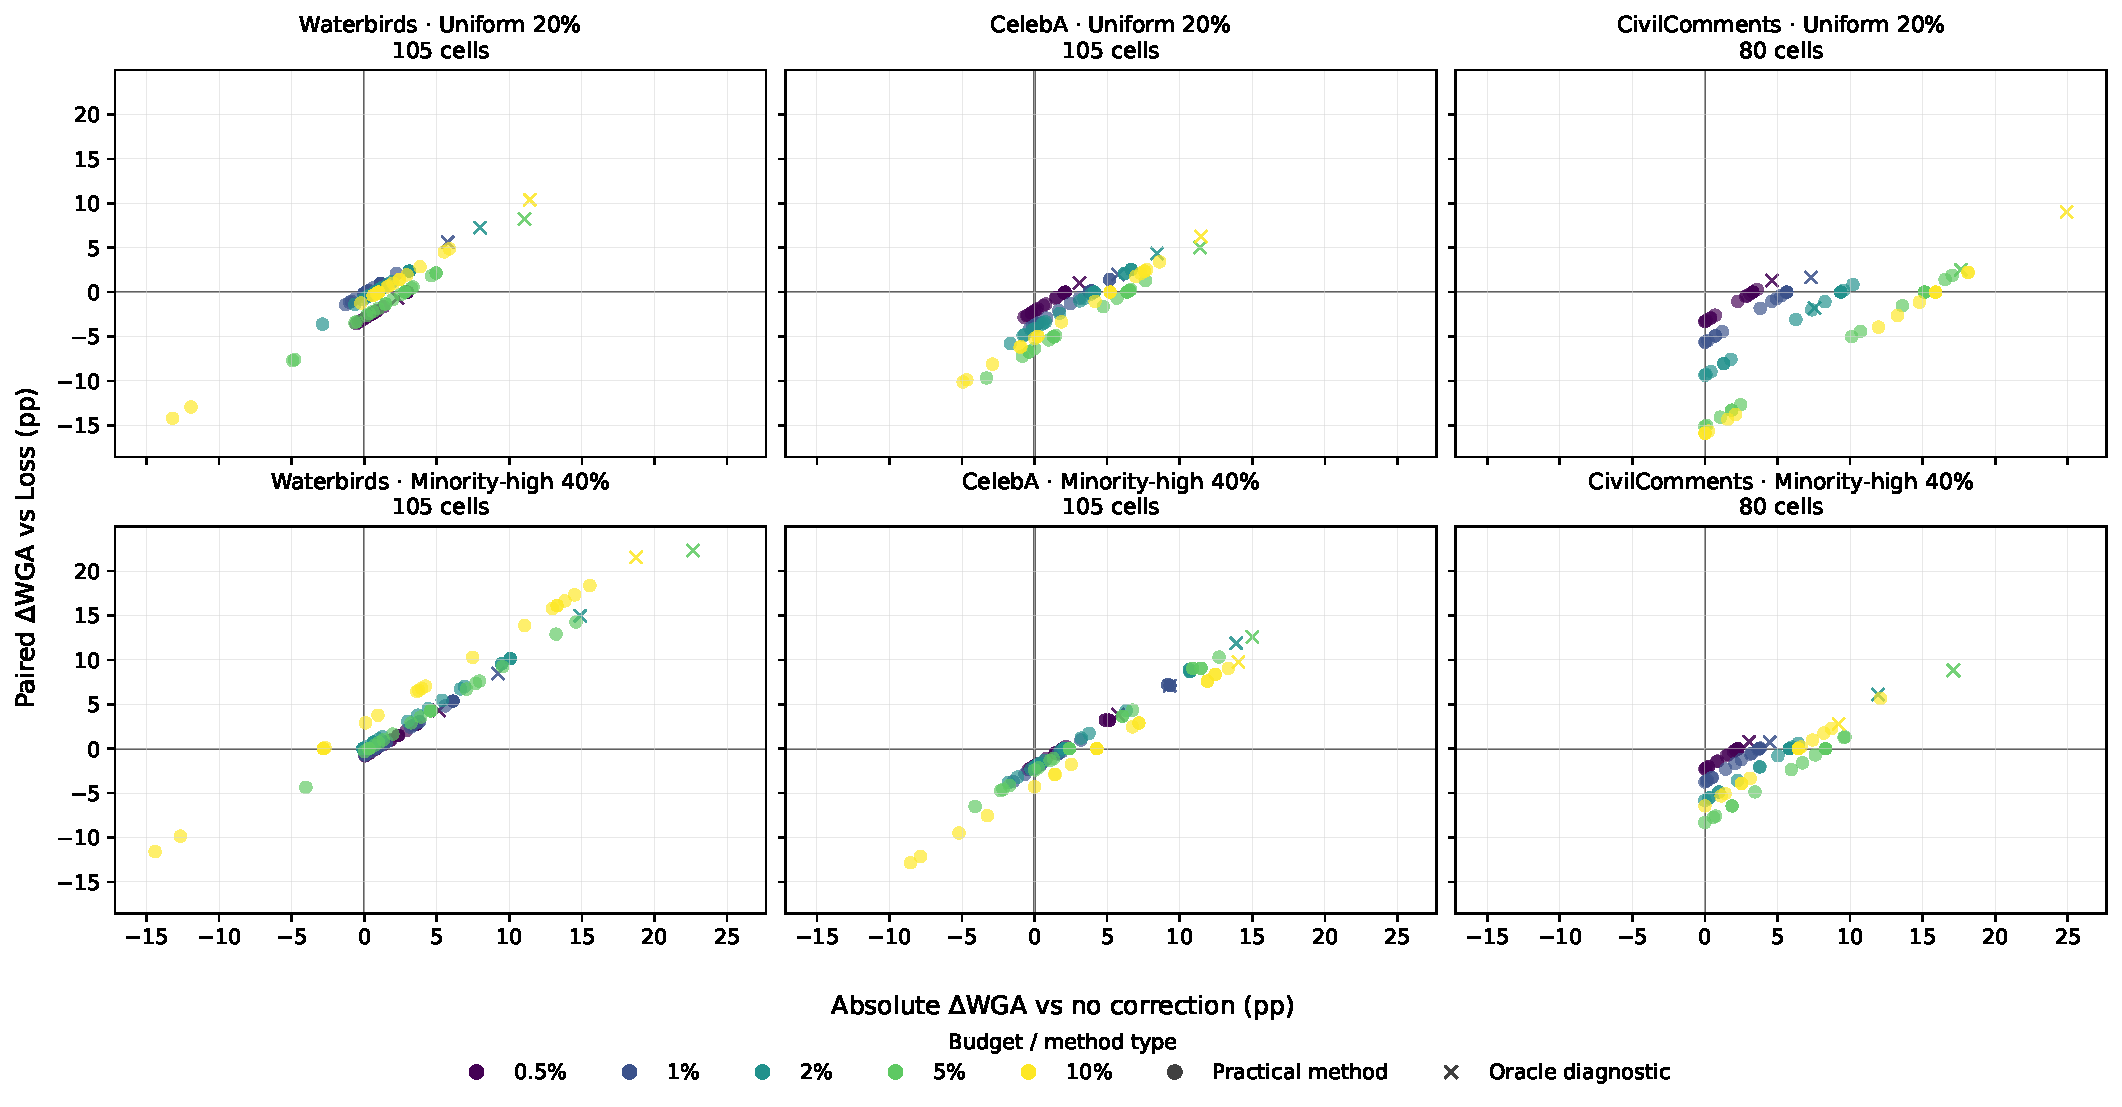
\includegraphics[width=\textwidth]{figures_diagnostic/fig3_complete_matrix_overview.pdf}
\caption[All 580 aggregate cells in the frozen-feature matrix.]{\raggedright All 580 aggregate cells in the frozen-feature matrix. Each point is one dataset/noise/method/budget cell; circles are practical methods and crosses are oracle diagnostics. Absolute utility and the paired contrast against Loss are shown separately.\par}
  \label{fig:matrix-overview}
\end{figure}

\subsection{A frozen counterexample and attribution screen}

\begin{table}[H]
\caption{CelebA uniform20 at a $10\%$ budget. Intervals are ten-seed 95\% $t$ intervals; all values except correction counts are pp.}
\centering
\scriptsize
\setlength{\tabcolsep}{2.2pt}
\resizebox{\textwidth}{!}{%
\begin{tabular}{lrrrrrr}
\toprule
Method & \shortstack{$\dwga$ vs\\no correction} & \shortstack{$\dwga$ vs\\Loss} & \shortstack{$\Delta$ precision\\vs Loss} & \shortstack{$\Delta$ corrected\\vs Loss} & \shortstack{$\Delta$ minority query\\rate vs Loss} & Neg. seeds \\
\midrule
Loss & $+5.21\;[+3.43,+6.98]$ & reference & reference & reference & reference & $0/10$ \\
TracIn-CP (val) & $-4.92\;[-7.41,-2.44]$ & $-10.13\;[-12.55,-7.71]$ & $+0.29\;[+0.21,+0.37]$ & $+46.5\;[+33.4,+59.6]$ & $-0.91\;[-1.03,-0.79]$ & $10/10$ \\
NoiseScore & $+7.73\;[+6.24,+9.22]$ & $+2.52\;[+0.72,+4.33]$ & $-89.44\;[-89.92,-88.96]$ & $-14558.1\;[-14636.9,-14479.3]$ & $+0.85\;[+0.62,+1.09]$ & $0/10$ \\
\bottomrule
\end{tabular}}
\end{table}

The attribution screen reinforces the same separation. Single- and multi-checkpoint TracIn have $99.33\%$ and $99.16\%$ query precision but negative \dwga{} in all seeds, whereas RV-Q and an action-space adaptation of AUTO-D3M have lower precision and positive WGA. These rows diagnose allocation rather than add evidence for the CelebA full-retraining comparison.

\begin{table}[H]
\caption{Frozen-feature attribution screen. Intervals are seed-bootstrap intervals. AUTO-D3M-Q is a query-action adaptation, not a reproduction of the original deletion method.}
\centering
\scriptsize
\begin{tabular}{lrrrr}
\toprule
Method & $\Delta$WGA (pp) & vs. Loss (pp) & Noise prec. (\%) & Neg. seeds \\
\midrule
Loss & +4.84 [+3.39, +5.94] & -- & 99.31 & 1/10 \\
TracIn-CP (single) & -6.62 [-8.01, -5.40] & -11.45 [-12.33, -10.60] & 99.33 & 10/10 \\
TracIn-CP (multi) & -8.07 [-9.69, -6.62] & -12.90 [-13.75, -12.05] & 99.16 & 10/10 \\
RV-Q (tail-product) & +8.31 [+7.59, +8.94] & +3.47 [+2.56, +4.45] & 6.59 & 0/10 \\
AUTO-D3M-Q (adapt.) & +12.29 [+11.65, +12.92] & +7.45 [+6.34, +8.64] & 12.76 & 0/10 \\
\bottomrule
\end{tabular}

\end{table}

\subsection{Validation quality and tail-fraction sensitivity}
\label{app:rv-sensitivity}

To test the inputs to RV-Q, we vary the validation-tail fraction, validation-pool size, and validation-label quality on the CelebA frozen-feature screen. The retraining and evaluation rule is held fixed, and each row changes one factor from the clean full-pool reference ($\tau=0.20$).

\begin{table}[H]
\caption{RV-Q validation sensitivity on CelebA frozen features. Means are over ten seeds; accuracy changes and paired gains are percentage points. ``Positive'' counts seeds with RV-Q paired $\dwga{}$ above Loss.}
\label{tab:rv-sensitivity}
\centering
\scriptsize
\setlength{\tabcolsep}{2.1pt}
\resizebox{\textwidth}{!}{%
\begin{tabular}{cccrrrrr}
\toprule
$\tau$ & Val. fraction & Val. noise & \shortstack{$\dwga$ vs\\no correction} & \shortstack{RV-Q $-$ Loss\\$\dwga$} & \shortstack{Query\\precision} & \shortstack{Val. label\\accuracy} & Positive \\
\midrule
0.05 & 1.00 & $0\%$ & $+7.17$ & $+2.33$ & $4.98\%$ & $100.00\%$ & $9/10$ \\
0.10 & 1.00 & $0\%$ & $+7.77$ & $+2.93$ & $5.83\%$ & $100.00\%$ & $10/10$ \\
0.20 & 0.10 & $0\%$ & $+8.18$ & $+3.34$ & $6.49\%$ & $100.00\%$ & $10/10$ \\
0.20 & 0.25 & $0\%$ & $+8.31$ & $+3.47$ & $6.54\%$ & $100.00\%$ & $10/10$ \\
0.20 & 0.50 & $0\%$ & $+8.59$ & $+3.75$ & $6.68\%$ & $100.00\%$ & $10/10$ \\
0.20 & 1.00 & $0\%$ & $+8.31$ & $+3.47$ & $6.59\%$ & $100.00\%$ & $10/10$ \\
0.20 & 1.00 & $5\%$ & $+3.45$ & $-1.39$ & $1.76\%$ & $95.00\%$ & $2/10$ \\
0.20 & 1.00 & $10\%$ & $+3.35$ & $-1.48$ & $1.68\%$ & $90.00\%$ & $2/10$ \\
0.20 & 1.00 & $20\%$ & $+3.21$ & $-1.63$ & $1.58\%$ & $80.00\%$ & $2/10$ \\
0.30 & 1.00 & $0\%$ & $+8.56$ & $+3.72$ & $6.96\%$ & $100.00\%$ & $10/10$ \\
0.40 & 1.00 & $0\%$ & $+8.65$ & $+3.82$ & $7.25\%$ & $100.00\%$ & $10/10$ \\
0.50 & 1.00 & $0\%$ & $+8.90$ & $+4.07$ & $7.50\%$ & $100.00\%$ & $10/10$ \\
\bottomrule
\end{tabular}}
\end{table}

With clean validation labels, the paired gain rises from $+2.33$ pp at $\tau=0.05$ to $+4.07$ pp at $\tau=0.50$ and remains positive in at least $9/10$ seeds. Reducing the pool from $100\%$ to $10\%$ changes the gain only from $+3.47$ to $+3.34$ pp. Label quality is the sharper boundary: $5$--$20\%$ validation corruption lowers precision from $6.59\%$ to $1.58$--$1.76\%$ and reverses the paired advantage to $-1.39$--$-1.63$ pp. Thus clean validation labels are a substantive assumption, not a cosmetic implementation choice.

\subsection{Young/Male full-retraining tail sensitivity}
\label{app:young-male-tau}

Figure~\ref{fig:young-male-tau} varies the validation-tail fraction over $\tau\in\{0.05,0.10,0.20,0.30,0.50\}$ while holding the Young/Male data, query budget, and retraining setup fixed. The mean absolute effects are $-1.38$, $+0.51$, $+2.45$, $+5.94$, and $+5.86$ pp, respectively; the paired effects against Loss are $-1.86$, $+0.03$, $+1.97$, $+5.46$, and $+5.38$ pp. The wider tails produce the largest gains, with similar means at $\tau=0.30$ and $0.50$.

\begin{figure}[H]
  \centering
  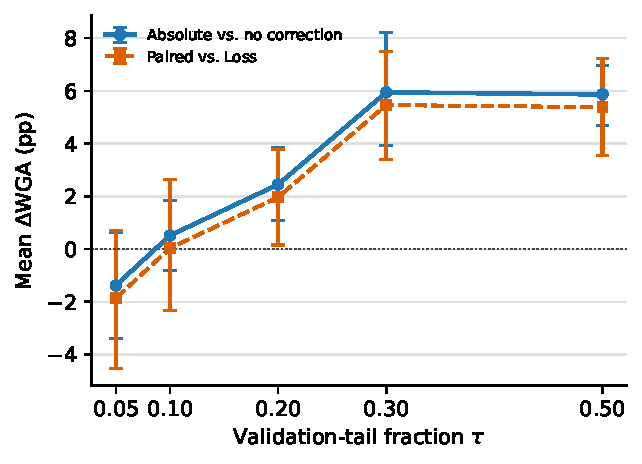
\includegraphics[width=0.62\textwidth]{figures_diagnostic/fig_young_male_tau_sensitivity.pdf}
  \caption{CelebA Young/Male full-retraining sensitivity over the validation-tail fraction. Points are means over 20 seeds and bars are 95\% seed-bootstrap intervals. The absolute curve compares with no correction; the paired curve compares with the same-seed Loss baseline.}
  \label{fig:young-male-tau}
\end{figure}

\subsection{Waterbirds full-retraining tail sensitivity}
\label{app:waterbirds-fulltrain-tau}

We vary $\tau\in\{0.20,0.30,0.35,0.40,0.50\}$ on the same Waterbirds full-retraining block while holding all other settings fixed. Figure~\ref{fig:waterbirds-fulltrain-tau} and Table~\ref{tab:waterbirds-fulltrain-tau} show a broad positive plateau over $\tau=0.35$--$0.50$. The main text reports $\tau=0.35$, which has the largest mean; it exceeds $\tau=0.50$ by $+0.022$ pp $[-0.734,+0.824]$ in a seed-paired comparison.

\begin{figure}[H]
  \centering
  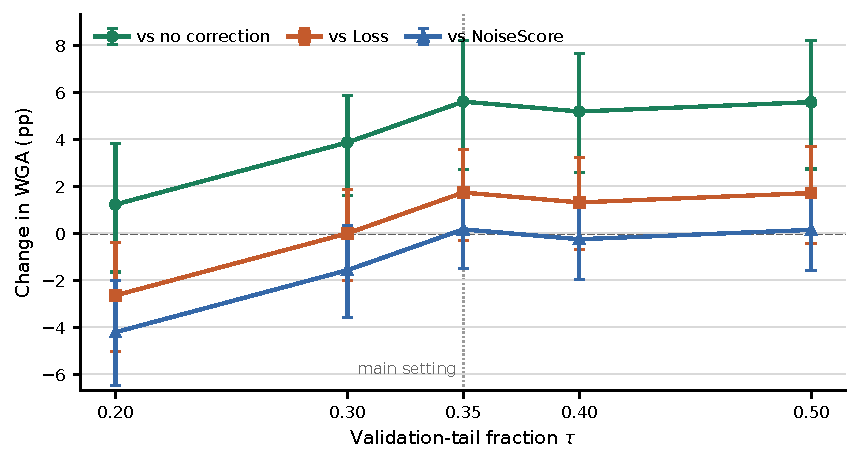
\includegraphics[width=0.70\textwidth]{figures_diagnostic/fig_waterbirds_fulltrain_tau_sensitivity.pdf}
  \caption{Waterbirds full-retraining sensitivity over the validation-tail fraction. Points are means over 20 seeds and bars are 95\% seed-bootstrap intervals. Curves report the absolute effect relative to no correction and paired effects relative to Loss and NoiseScore.}
  \label{fig:waterbirds-fulltrain-tau}
\end{figure}

\begin{table}[H]
\caption{Waterbirds full-retraining tail sensitivity. Effects are percentage-point means with 95\% seed-bootstrap intervals. Positive counts are reported as absolute/Loss/NoiseScore.}
\label{tab:waterbirds-fulltrain-tau}
\centering
\scriptsize
\setlength{\tabcolsep}{3.0pt}
\begin{tabular}{ccccc}
\toprule
$\tau$ & Absolute $\dwga$ & RV-Q $-$ Loss & RV-Q $-$ NoiseScore & Positive seeds \\
\midrule
0.20 & $+1.23\;[-1.65,+3.83]$ & $-2.64\;[-5.04,-0.40]$ & $-4.21\;[-6.48,-2.00]$ & $13/6/5$ \\
0.30 & $+3.86\;[+1.60,+5.87]$ & $-0.00\;[-2.00,+1.86]$ & $-1.57\;[-3.60,+0.35]$ & $17/11/9$ \\
0.35 & $+5.60\;[+2.72,+8.21]$ & $+1.73\;[-0.30,+3.58]$ & $+0.17\;[-1.48,+1.70]$ & $18/14/12$ \\
0.40 & $+5.18\;[+2.57,+7.65]$ & $+1.31\;[-0.68,+3.23]$ & $-0.25\;[-1.96,+1.38]$ & $17/13/12$ \\
0.50 & $+5.58\;[+2.74,+8.20]$ & $+1.71\;[-0.45,+3.69]$ & $+0.15\;[-1.57,+1.77]$ & $18/13/12$ \\
\bottomrule
\end{tabular}
\end{table}

\subsection{Waterbirds RV-Q-Gated tail sensitivity}
\label{app:waterbirds-gated-tau}

On the disjoint Waterbirds seeds 40--59, we evaluate the gated rule at
$\tau=0.20$, $0.30$, $0.35$, $0.40$, and $0.50$, keeping the $0.50$ NoiseScore anchor,
$2B$ candidate pool, data split, and query budget fixed. The gated rule is
therefore evaluated as a tail-fraction ablation rather than as a single
preselected setting. This auxiliary frozen-feature linear-head block is separate from the end-to-end
comparison reported above. We select the displayed setting from the highest
mean validation balanced accuracy, which is available before test evaluation;
validation selects $\tau=0.40$. Across the five settings, mean absolute
$\dwga$ changes range from $-5.83$ to $-4.60$ pp, while paired differences
against NoiseScore range from $+0.25$ to $+1.48$ pp. The complete seed-level
sensitivity is reported below.

\begin{figure}[H]
  \centering
  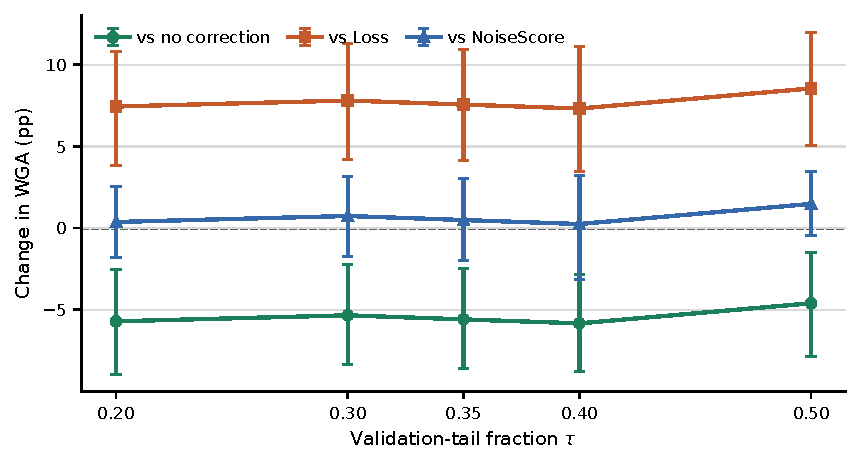
\includegraphics[width=0.70\textwidth]{figures_diagnostic/fig_waterbirds_gated_tau_sensitivity.pdf}
  \caption{Waterbirds RV-Q-Gated frozen-feature linear-head sensitivity over the validation-tail fraction on seeds 40--59. Points are seed means and bars are 95\% seed-bootstrap intervals. Curves report absolute effects relative to no correction and paired effects relative to Loss and NoiseScore.}
  \label{fig:waterbirds-gated-tau}
\end{figure}

\begin{table}[H]
\caption{Waterbirds RV-Q-Gated frozen-feature linear-head tail-fraction sensitivity on seeds 40--59. Effects are percentage-point means with 95\% seed-bootstrap intervals. Positive counts are reported as absolute/Loss/NoiseScore.}
\label{tab:waterbirds-gated-tau}
\centering
\scriptsize
\setlength{\tabcolsep}{3.0pt}
\begin{tabular}{ccccc}
\toprule
$\tau$ & Absolute $\dwga$ & RV-Q-Gated $-$ Loss & RV-Q-Gated $-$ NoiseScore & Positive seeds \\
\midrule
0.20 & $-5.71\;[-8.95,-2.54]$ & $+7.44\;[+3.83,+10.83]$ & $+0.37\;[-1.79,+2.54]$ & 5/18/11 \\
0.30 & $-5.34\;[-8.37,-2.20]$ & $+7.81\;[+4.20,+11.30]$ & $+0.74\;[-1.73,+3.19]$ & 6/18/12 \\
0.35 & $-5.59\;[-8.61,-2.45]$ & $+7.56\;[+4.11,+10.94]$ & $+0.49\;[-2.01,+3.02]$ & 5/18/11 \\
0.40 & $-5.83\;[-8.76,-2.87]$ & $+7.32\;[+3.47,+11.11]$ & $+0.25\;[-3.13,+3.24]$ & 5/17/12 \\
0.50 & $-4.60\;[-7.86,-1.48]$ & $+8.55\;[+5.08,+11.98]$ & $+1.48\;[-0.47,+3.47]$ & 6/17/13 \\
\bottomrule
\end{tabular}
\end{table}


\subsection{20-seed Waterbirds frozen-feature extension}
\label{app:rv-waterbirds-20}

This extension is separate from the Waterbirds full-retraining blocks. It compares
Loss, NoiseScore, Entropy, and RV-Q at budgets $2\%$ and $5\%$ and tail fractions
$\tau\in\{0.20,0.50\}$ over 20 seeds, using the same frozen-feature linear-head
evaluation throughout. The table below reports the complete RV-Q summary.

\begin{table}[H]
\caption{Full 20-seed Waterbirds extension summary. Values are mean absolute or paired effects in pp; intervals are 10,000-replicate percentile bootstrap intervals over seeds. The Entropy comparison is available in the released CSV but omitted here for space.}
\label{tab:rv-waterbirds-20-full}
\centering
\scriptsize
\setlength{\tabcolsep}{2.2pt}
\resizebox{\textwidth}{!}{%
\begin{tabular}{llrrrrrr}
\toprule
Noise & Budget & $\tau$ & Abs. mean & Abs. CI low & Abs. CI high & RV-Q$-$Loss & RV-Q$-$NoiseScore \\
\midrule
uniform20 & $2\%$ & 0.20 & $+2.76$ & $+1.30$ & $+4.89$ & $+1.65\;[+0.19,+3.08]$ & $+1.16\;[-1.27,+3.44]$ \\
uniform20 & $5\%$ & 0.20 & $+1.81$ & $-1.04$ & $+4.88$ & $+4.32\;[+0.56,+7.68]$ & $+4.61\;[+0.15,+8.80]$ \\
uniform20 & $2\%$ & 0.50 & $+6.72$ & $+4.63$ & $+9.13$ & $+5.62\;[+2.14,+8.61]$ & $+5.12\;[+1.74,+8.00]$ \\
uniform20 & $5\%$ & 0.50 & $+7.06$ & $+4.50$ & $+9.63$ & $+9.56\;[+6.76,+12.13]$ & $+9.85\;[+7.24,+12.37]$ \\
minority-high-40 & $2\%$ & 0.20 & $-0.55$ & $-3.07$ & $+1.50$ & $+4.78\;[+1.29,+8.32]$ & $-6.34\;[-9.96,-3.14]$ \\
minority-high-40 & $5\%$ & 0.20 & $+1.19$ & $-1.75$ & $+3.64$ & $+9.38\;[+7.09,+11.80]$ & $-8.53\;[-11.24,-5.96]$ \\
minority-high-40 & $2\%$ & 0.50 & $+3.88$ & $+0.33$ & $+7.20$ & $+9.21\;[+6.36,+12.07]$ & $-1.92\;[-5.81,+1.10]$ \\
minority-high-40 & $5\%$ & 0.50 & $+8.51$ & $+5.96$ & $+11.20$ & $+16.71\;[+13.45,+20.03]$ & $-1.21\;[-3.92,+1.40]$ \\
\bottomrule
\end{tabular}}
\end{table}

All rankings use legal pre-query observables; clean training and group labels enter
only the post-query diagnostics. Absolute effects are measured against the
same-seed no-query model and paired effects against the corresponding reference.

\subsection{CelebA seed-level contrast}

The seed-level values behind the main CelebA comparison are shown in Table~\ref{tab:perseed-rv}. They make the paired result transparent: the RV-Q advantage is positive in nine of ten non-tied seeds, with one small negative seed in absolute utility.

\begin{table}[H]
\caption{RV-Q (tail-product) held-out test on CelebA seeds 20--29. Values are absolute \dwga{} and the paired contrast against Loss, in pp.}
\label{tab:perseed-rv}
\centering
\small
\resizebox{\textwidth}{!}{%
\begin{tabular}{rrrrrrrrrrr}
\toprule
Seed & 20 & 21 & 22 & 23 & 24 & 25 & 26 & 27 & 28 & 29 \\
\midrule
RV-Q abs. & $+0.631$ & $+0.946$ & $+0.253$ & $-0.315$ & $-0.309$ & $+0.055$ & $+0.782$ & $+1.577$ & $+0.061$ & $+0.631$ \\
Loss abs. & $+0.315$ & $-0.631$ & $-1.262$ & $-0.315$ & $-1.721$ & $-0.315$ & $-0.042$ & $+0.315$ & $-1.577$ & $-0.315$ \\
Paired & $+0.315$ & $+1.577$ & $+1.515$ & $0.000$ & $+1.412$ & $+0.370$ & $+0.823$ & $+1.262$ & $+1.639$ & $+0.946$ \\
\bottomrule
\end{tabular}}
\end{table}

The baseline worst group is group 2 in nine RV-Q seeds and group 3 in one. Descriptively, those groups contain 5,598 corrupted training examples across seeds: RV-Q repairs 5,538, Loss 2,675, Random 595, and TracIn zero. Inference remains seed-level; these pooled counts only expose the composition pattern.

\subsection{Waterbirds held-out follow-up}

\begin{table}[H]
\caption{Waterbirds uniform20, 10\% end-to-end follow-up. Values are absolute \dwga{} in pp for seeds 10--19. The block is descriptive and external-validity evidence only.}
\centering
\small
\resizebox{\textwidth}{!}{%
\begin{tabular}{lrrrrrrrrrr}
\toprule
Method & 10 & 11 & 12 & 13 & 14 & 15 & 16 & 17 & 18 & 19 \\
\midrule
Random & $+1.552$ & $+1.402$ & $+7.321$ & $+2.960$ & $+2.181$ & $+5.603$ & $+13.084$ & $+1.558$ & $+3.583$ & $+0.312$ \\
Loss & $+8.684$ & $+8.879$ & $+6.542$ & $+9.376$ & $-2.960$ & $+4.982$ & $+11.371$ & $-2.025$ & $0.000$ & $+10.220$ \\
TracIn & $+1.363$ & $+4.206$ & $+9.346$ & $+12.461$ & $-8.411$ & $-5.452$ & $+4.361$ & $-20.717$ & $+4.361$ & $+3.583$ \\
\bottomrule
\end{tabular}}
\end{table}

Random is positive in all ten seeds and has mean absolute \dwga{} $+3.955$ pp $[+1.992,+6.448]$. Loss has mean $+5.507$ pp $[+2.242,+8.463]$ but only $7$ positive, $2$ negative, and $1$ tied seed. TracIn has mean $+0.510$ pp with a wide interval and severe negative outliers. The bootstrap mean contrast favors Loss over TracIn, but the exact sign test is $p=0.34375$; this is magnitude-based, heterogeneous evidence rather than sign-stable confirmation.

\subsection{Waterbirds RV-Q transfer blocks}

\begin{figure}[H]
  \centering
  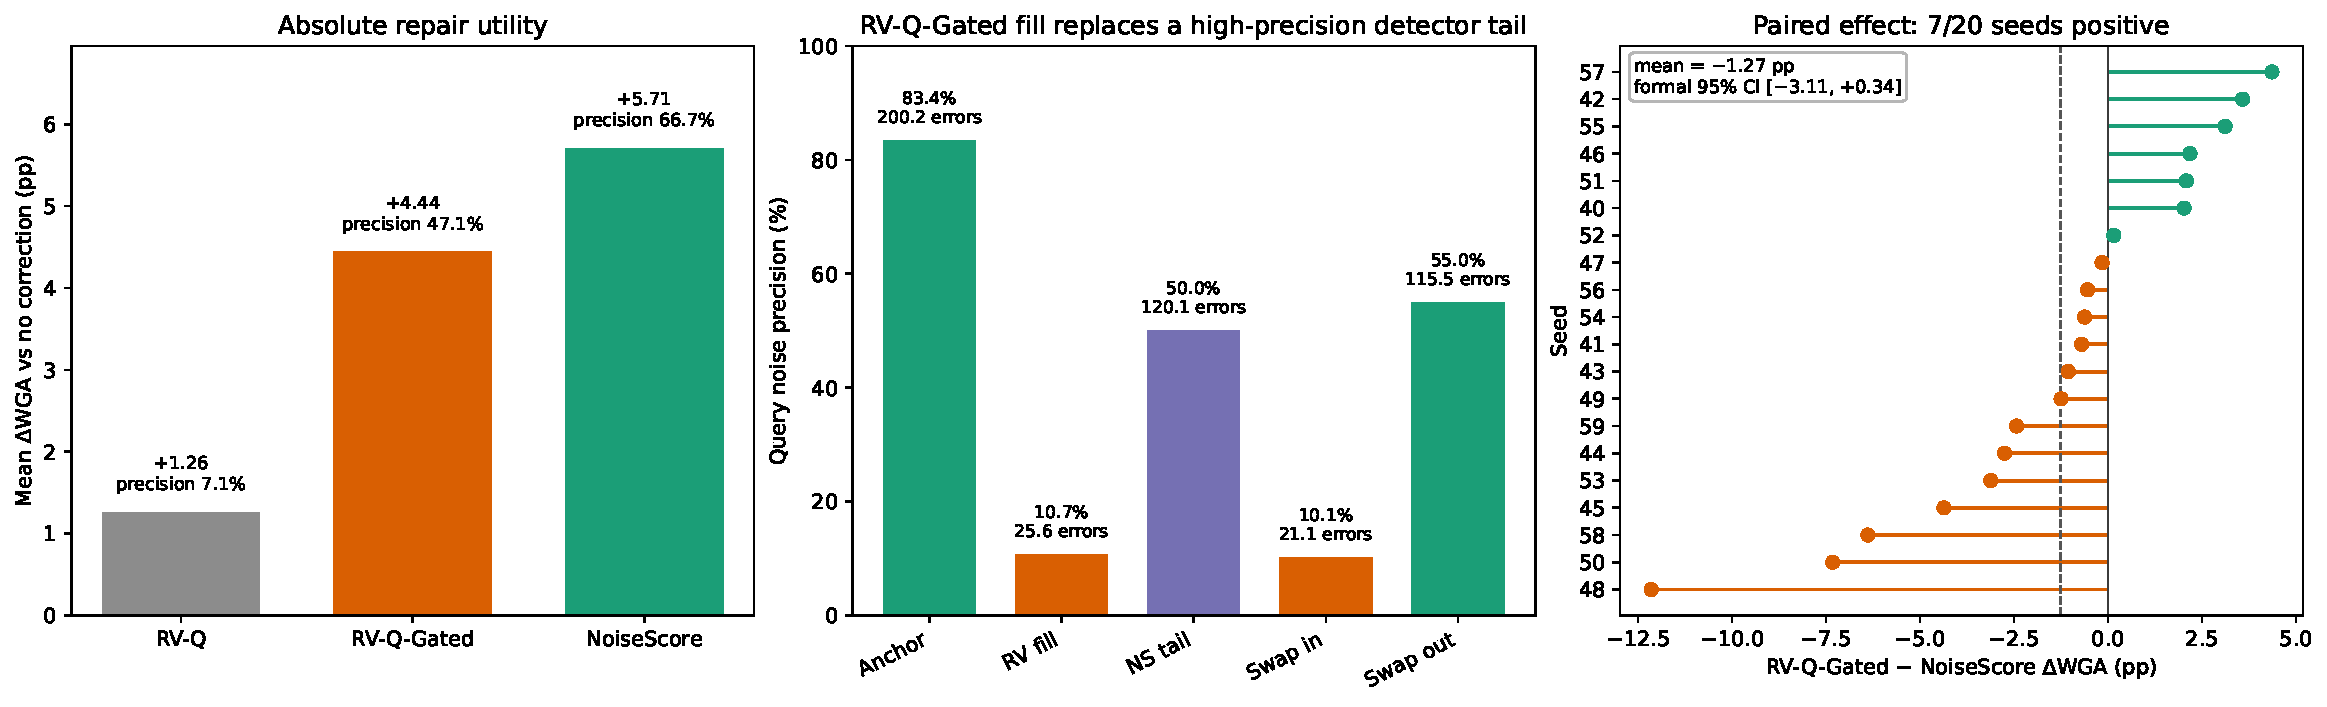
\includegraphics[width=\textwidth]{figures_diagnostic/fig4_waterbirds_v2_mechanism.pdf}
  \caption{Waterbirds RV-Q-Gated audit, seeds 40--59. Left: RV-Q-Gated improves absolute WGA but has a $1.27$ pp lower paired point estimate than NoiseScore. Middle: the anchor stage exactly preserves the NoiseScore prefix, whereas the RV-Q tail-value fill has $10.67\%$ precision and displaces a $50.04\%$-precision NoiseScore tail. Right: the paired effect favors NoiseScore in 13/20 seeds.}
  \label{fig:waterbirds-v2}
\end{figure}

At $\tau=0.20$, the initial RV-Q block on seeds 20--39 has absolute utility $+1.226$ pp $[-1.647,+3.830]$ and a $-2.642$ pp paired comparison against Loss $[-5.038,-0.399]$, with $6/20$ positive paired seeds. The full sensitivity in Appendix~\ref{app:waterbirds-fulltrain-tau} shows that this comparison changes across the tail range.

The RV-Q-Gated block covers the disjoint seeds 40--59 and compares against NoiseScore. It keeps a $0.50$ NoiseScore anchor and varies the validation-tail fraction of the repair-value fill; the complete sensitivity is reported in Appendix~\ref{app:waterbirds-gated-tau}. The appendix reports the validation-selected setting and the full tail curve; the end-to-end comparison remains the transfer result above.

\begin{table}[H]
\caption{Additional Waterbirds transfer blocks. Values are percentage points (pp) except precision; intervals are 95\% seed-bootstrap intervals.}
\label{tab:e2e-waterbirds-appendix}
\centering
\scriptsize
\setlength{\tabcolsep}{2.2pt}
\resizebox{\textwidth}{!}{%
\begin{tabular}{p{0.23\textwidth}p{0.21\textwidth}p{0.21\textwidth}p{0.11\textwidth}p{0.14\textwidth}}
\toprule
Evidence block & Paired effect & Absolute $\dwga$ & Precision & Seeds $(+/-/tie)$ \\
\midrule
TracIn, 10--19 & Loss: $-5.00\;[-9.21,-0.96]$ & $+0.51\;[-5.60,+5.70]$ & $84.81\%$ & $7/3/0$ \\
RV-Q, 20--39 ($\tau=.20$) & Loss: $-2.64\;[-5.04,-0.40]$ & $+1.23\;[-1.65,+3.83]$ & $5.59\%$ & $6/14/0$ \\
RV-Q-Gated, 40--59 (anchor $=.50$) & NoiseScore: $-1.27\;[-3.11,+0.34]$ & $+4.44\;[+1.29,+7.65]$ & $47.05\%$ & $7/13/0$ \\
\bottomrule
\end{tabular}
}
\end{table}

\subsection{Model references and baseline supplement}
\label{app:baselines}

\subsubsection{RV-Q pseudocode}
\label{app:rvq-algorithm}

The implementation uses a class-balanced CVaR-style validation tail. For class
$c$, let $T_c$ contain the highest-loss fraction $	au$ of validation examples
with observed clean class $c$ and set
\begin{equation}
  w_j=\frac{1}{C|T_c|}\mathbf 1\{j\in T_c\},\qquad
  g_c=\sum_j w_j\big(q_{jc}-\mathbf 1\{y_j^v=c\}\big)\phi(x_j^v),
  \label{eq:rvq-tail-grad-appendix}
\end{equation}
where the tail threshold is the $(1-\tau)$ loss quantile within class $c$.
For binary labels, Eq.~\ref{eq:repairvalue} uses the gradient difference
$g_0-g_1$; the multiclass posterior-marginalized extension is in
Appendix~\ref{app:cifar10n}.

\begin{algorithm}[H]
\caption{RV-Q as a preliminary value-alignment baseline}
\label{alg:repairvalue-appendix}
\begin{algorithmic}[1]
\Require Noisy training set $\mathcal D$, frozen features $\phi(x_i)$, validation set $\mathcal V$ with features and linear-head probabilities, detector scores $\rho_i$, budget $B$, tail fraction $\tau$
\Ensure Query set $Q$ and retrained model $f_Q$
\State Compute class-conditional tail weights $w_j$ at fraction $\tau$
\State Compute class gradients $g_c$ for all classes $c=0,\ldots,C-1$ from the tail weights above
\State Compute $\hat v_i$ from Eq.~\ref{eq:repairvalue}; for $C>2$, use Appendix~\ref{app:cifar10n}
\State Rank-normalize $\{\hat v_i\}$ to $r_i\in[0,1]$
\State Form scores $s_i\leftarrow \rho_i r_i$ and break ties by $\rho_i$, then loss
\State Select $Q\leftarrow$ top-$B$ scored examples
\State Review $Q$, replace $\tilde y_i$ with $y_i$ for $i\in Q$
\State Retrain on the corrected training set to obtain $f_Q$
\State \Return $Q$ and the retrained model $f_Q$
\end{algorithmic}
\end{algorithm}

\subsubsection{Query and model references}

\paragraph{Baseline nomenclature and scope.}
The following definitions make the method names in the frozen matrix and the
baseline supplement unambiguous. Practical rows use only pre-query observables;
oracle rows are offline diagnostics.

\begin{table}[H]
\caption{Baseline taxonomy and operational definitions.}
\label{tab:baseline-taxonomy}
\centering
\scriptsize
\setlength{\tabcolsep}{2.5pt}
\begin{tabular}{p{0.20\textwidth}p{0.47\textwidth}p{0.24\textwidth}}
\toprule
Method & Query rule used in this audit & Role and information status \\
\midrule
Random & Uniform sampling without replacement; the seed controls the permutation. & Practical reference. \\
Loss & Descending final-probe cross-entropy on the observed noisy label; ties use the stable sample order. & Practical detection reference. \\
Entropy & Descending predictive entropy of the final probe, with loss as a tie-breaker. & Practical uncertainty reference. \\
NoiseScore & Descending supplied label-noise proxy from the probe/dynamics pipeline, with loss as a tie-breaker. & Practical detector reference; the score is not a clean-label or group oracle. \\
ND / NN-Agree & Descending neighborhood disagreement among the 20 cosine-nearest frozen-feature neighbors, with loss as a tie-breaker. & Practical local-consistency detector; no group labels. \\
kNN-LS-Q (adapt.) & Descending soft kNN pseudo-label disagreement plus entropy; only selected labels are reviewed and corrected. & Query-action adaptation of NeurIPS 2024 label spreading \citep{stromberg2024enhancing}; not an automatic relabeling reproduction. \\
BHC / NGC & BHC adds budget-triggered cluster-coverage diversification to NoiseScore. NGC preserves NoiseScore at budgets at or below $2\%$; above that it uses coverage only when the top-$B$/overall loss ratio is at most $4.0$. & Practical coverage baselines; no group labels. \\
CPBA family & CPBA reweights NoiseScore by the observed noisy-label class's mean loss; CPBA-only has no coverage or fallback, while CPBA-TC variants add coverage and specify their fallback policy. & Allocation diagnostics; separate from RV-Q. \\
RV-Q & Clipped NoiseScore proxy multiplied by the normalized class-balanced validation-tail repair-value rank. & Initial value-alignment baseline; no group labels and no universal guarantee. \\
RV-Q (multiclass) & Uses the same noise proxy with a posterior-marginalized repair-value rank over all candidate clean classes. & Mechanical multiclass scope check; no group labels. \\
RV-Q-Gated & Keeps a NoiseScore anchor prefix and fills the remaining budget with tail repair-value ranking inside a NoiseScore candidate pool. & Separate failure-probe variant. \\
TracIn-CP & TracIn-CP (val) uses one final checkpoint; TracIn-CP (multi) averages influence over observed checkpoints; TracIn-CP (noise) multiplies normalized validation-uncertainty influence by NoiseScore. & Practical attribution baselines; adaptations are not WGA oracles. \\
Cleanlab / active cleaning & In-sample or five-fold OOF confident-learning priorities; frozen-feature expected-model-change; or CE-minus-entropy one-shot priority. & Mainstream practical baselines, explicitly labeled adaptations where applicable. \\
Oracle diagnostics & Use clean noise/group information or group-aware retraining only for counterfactual references and failure diagnostics. & Not legal query rules and never pooled with practical methods. \\
\bottomrule
\end{tabular}
\end{table}

The complete frozen matrix also includes the following classical proxies (grouped
here to keep the result tables readable).
Forgetting counts correct-to-incorrect transitions in the probe trajectory;
AUM ranks by the mean training margin (lower first); and Margin ranks by the
final noisy-label margin (lower first), with final loss as a tie-breaker.

\paragraph{Neighborhood disagreement and label spreading.}
Let $\mathcal N_{20}(i)$ be the 20 nearest examples other than $i$ under cosine
distance between frozen features. ND, reported in result files as NN-Agree,
uses
\begin{equation}
 s_i^{\mathrm{ND}}=1-\frac1{20}\sum_{j\in\mathcal N_{20}(i)}
 \mathbf 1\{\tilde y_j=\tilde y_i\},
 \label{eq:nd}
\end{equation}
with descending priority and final loss as the tie-breaker. For kNN-LS-Q, let
$w_{ij}=\exp(\cos(\phi_i,\phi_j)/0.5)$ and
\begin{equation}
 \hat p_{ic}=\frac{\sum_{j\in\mathcal N_{20}(i)}w_{ij}
 \mathbf 1\{\tilde y_j=c\}}{\sum_{j\in\mathcal N_{20}(i)}w_{ij}},\qquad
 s_i^{\mathrm{LSQ}}=1-\hat p_{i\tilde y_i}
 +0.3R\!\left(H(\hat p_i)\right),
 \label{eq:lsq}
\end{equation}
where $R$ is the global tie-aware percentile rank. The top-$B$ examples are
reviewed; the pseudo-labels themselves never replace training labels.
Stromberg et al. instead use Euclidean $k$NN, a uniform majority vote, and one
round that overwrites the full training-label vector before RAD/SELF
last-layer correction \citep{stromberg2024enhancing}. Thus our row tests their
neighborhood intuition in a human-budgeted action space; it is not a reproduction
of their algorithm or training endpoint.

Coreset-Lite is a
scalable farthest-first (k-center) prefix on frozen features;
Unc+Div-Lite balances predictive entropy and feature distance with
$\beta=0.5$; and BADGE-Lite applies farthest-first selection to the gradient
embeddings $(p_i-e_{y_i})\otimes x_i$, seeded by loss.  NoiseScore+Cov and
NoiseScore+CluCov use predicted-class and representation-cluster buckets,
respectively, for warm-start coverage; their adaptive/gated versions switch
coverage as a function of budget.  TracIn-CP (noise) multiplies normalized
validation-uncertainty influence by NoiseScore.  These definitions use only
legal pre-query observables; the corresponding oracle TracIn and oracle-noise,
minority, disagreement, and group-balanced rankings read clean noise or group
labels and are therefore offline diagnostics rather than deployable baselines.

For completeness, CPBA (Class-Prior Balanced Allocation) uses the following
class weight. Let $K$ be the number of observed noisy-label classes,
$\bar\ell_c$ the mean final-probe loss in class $c$, and $\alpha$ the clipped
Spearman agreement between class-conditional and global loss ranks. For an
example with noisy label $y_i=c$, CPBA replaces the NoiseScore $\rho_i$ by

\begin{equation}
  \rho_i^{\mathrm{CPBA}}=\rho_i w_c,\qquad
  w_c=\operatorname{clip}_{[0.5,2]}
  \left[1+(1-\alpha)\left(
  \frac{\bar\ell_c/\sum_{c'}\bar\ell_{c'}}{1/K}-1\right)\right].
\end{equation}

The CPBA-only ranking is the descending order of $\rho_i^{\mathrm{CPBA}}$;
the CPBA-TC variants then apply their stated coverage and fallback modules.
The class labels here are the observed noisy labels, not hidden evaluation
groups. Thus CPBA is an allocation ablation, not a group-aware method and not
an alias for RV-Q.

\begin{table}[H]
\caption{Absolute references for the frozen linear-head evaluation. Values are ten-seed mean WGA (sem). Oracle GroupDRO uses private group labels and is an upper reference; JTT is a diagnostic for naive group-robust retraining under uniform label noise; headroom is the oracle gap in percentage points. \textbf{Takeaway:} JTT can collapse under noisy first-stage error sets, whereas the oracle gap quantifies the remaining repair headroom.}
\label{tab:absolute}
\centering
\scriptsize
\setlength{\tabcolsep}{1.8pt}
\begin{tabular}{llcccr}
\toprule
Dataset & Noise & No-query ERM & Oracle GroupDRO & JTT & \shortstack{Headroom\\(pp)} \\
\midrule
Waterbirds & uniform20 & $0.6081\;(0.0151)$ & $0.8249\;(0.0081)$ & $0.0573\;(0.0191)$ & $+21.7$ \\
Waterbirds & minority-high-40 & $0.4862\;(0.0189)$ & $0.6166\;(0.0189)$ & $0.3809\;(0.0129)$ & $+13.0$ \\
CelebA & uniform20 & $0.7628\;(0.0059)$ & $0.9096\;(0.0025)$ & $0.0004\;(0.0001)$ & $+14.7$ \\
CelebA & minority-high-40 & $0.6991\;(0.0078)$ & $0.7981\;(0.0105)$ & $0.2186\;(0.0272)$ & $+9.9$ \\
CivilComments & uniform20 & $0.0920\;(0.0019)$ & $0.6721\;(0.0026)$ & $0.0001\;(0.0000)$ & $+58.0$ \\
CivilComments & minority-high-40 & $0.0657\;(0.0011)$ & $0.6493\;(0.0043)$ & $0.0141\;(0.0004)$ & $+58.4$ \\
\bottomrule
\end{tabular}
\end{table}

The no-query ERM row defines the zero of every \dwga{}; Oracle GroupDRO is an
upper reference, never a legal query rule. Under uniform20, JTT's first-stage
error set is dominated by corrupted examples, and its upweighting collapses WGA
on CelebA and CivilComments.

\begin{table}[H]
\caption{Baseline-supplement query rules across budgets. Each cell is absolute $\dwga$ / paired $\dwga$ versus Loss in percentage points, averaged over seeds.}
\label{tab:supplement-full}
\centering
\scriptsize
\setlength{\tabcolsep}{2.2pt}
\resizebox{\textwidth}{!}{%
\begin{tabular}{llrrrrr}
\toprule
Noise & Method & 0.5\% & 1\% & 2\% & 5\% & 10\% \\
\midrule
\multicolumn{6}{l}{\emph{Waterbirds}} \\
uniform20 & Loss (reference) & +3.0/+0.0 & +0.1/+0.0 & +0.7/+0.0 & +2.8/+0.0 & +1.0/+0.0 \\
uniform20 & Cleanlab (in-sample) & +3.0/+0.0 & +0.1/+0.0 & +0.7/+0.0 & +2.8/+0.0 & +1.0/+0.0 \\
uniform20 & Cleanlab (OOF) & +1.8/-1.2 & +0.8/+0.7 & +0.8/+0.1 & +0.0/-2.8 & -1.8/-2.8 \\
uniform20 & ActiveClean (EMC adapt.) & -0.9/-3.8 & -2.0/-2.2 & -3.3/-4.0 & -4.0/-6.8 & -6.5/-7.5 \\
uniform20 & Active Label Cleaning & +3.0/+0.0 & +0.1/+0.0 & +0.7/+0.0 & +2.8/+0.0 & +1.0/+0.0 \\
uniform20 & NoiseScore & +0.5/-2.5 & +1.1/+1.0 & +3.1/+2.4 & +5.0/+2.2 & +0.6/-0.4 \\
uniform20 & RV-Q (tail-product) & +0.3/-2.7 & +0.8/+0.6 & +1.0/+0.3 & +2.6/-0.2 & +5.2/+4.2 \\
uniform20 & AUTO-D3M-Q (adapt.) & +4.1/+1.1 & +6.7/+6.6 & +8.6/+7.9 & +12.6/+9.8 & +14.4/+13.4 \\
uniform20 & TracIn-CP (val, multi) & +0.6/-2.4 & +0.6/+0.4 & -2.4/-3.2 & -5.6/-8.4 & -11.8/-12.8 \\
minority-high-40 & Loss (reference) & +0.8/+0.0 & +0.8/+0.0 & -0.1/+0.0 & +0.3/+0.0 & -2.8/+0.0 \\
minority-high-40 & Cleanlab (in-sample) & +0.8/+0.0 & +0.8/+0.0 & -0.1/+0.0 & +0.3/+0.0 & -2.8/+0.0 \\
minority-high-40 & Cleanlab (OOF) & +0.9/+0.1 & +2.1/+1.3 & +1.4/+1.5 & -3.0/-3.3 & -0.6/+2.2 \\
minority-high-40 & ActiveClean (EMC adapt.) & -0.8/-1.6 & -2.3/-3.1 & -5.8/-5.7 & -12.4/-12.7 & -5.6/-2.8 \\
minority-high-40 & Active Label Cleaning & +0.8/+0.0 & +0.8/+0.0 & -0.1/+0.0 & +0.3/+0.0 & -4.9/-2.1 \\
minority-high-40 & NoiseScore & +3.6/+2.7 & +6.1/+5.4 & +9.5/+9.5 & +4.6/+4.3 & +13.3/+16.1 \\
minority-high-40 & RV-Q (tail-product) & +3.2/+2.4 & +4.2/+3.4 & +6.7/+6.8 & +8.1/+7.8 & +9.1/+11.9 \\
minority-high-40 & AUTO-D3M-Q (adapt.) & +8.5/+7.7 & +11.1/+10.3 & +14.1/+14.2 & +17.2/+16.8 & +21.1/+23.9 \\
minority-high-40 & TracIn-CP (val, multi) & +0.5/-0.3 & +1.8/+1.1 & +0.3/+0.4 & -4.9/-5.2 & -13.1/-10.3 \\
\midrule
\multicolumn{6}{l}{\emph{CelebA}} \\
uniform20 & Loss (reference) & +2.1/+0.0 & +3.8/+0.0 & +4.1/+0.0 & +6.4/+0.0 & +5.2/+0.0 \\
uniform20 & Cleanlab (in-sample) & +2.1/+0.0 & +3.8/+0.0 & +4.1/+0.0 & +6.4/+0.0 & +5.2/+0.0 \\
uniform20 & Cleanlab (OOF) & +1.5/-0.6 & +2.0/-1.8 & +3.2/-0.9 & +3.7/-2.6 & +4.2/-1.0 \\
uniform20 & ActiveClean (EMC adapt.) & +0.7/-1.4 & +1.4/-2.4 & +2.0/-2.1 & +2.3/-4.1 & +2.6/-2.6 \\
uniform20 & Active Label Cleaning & +2.1/+0.0 & +3.8/+0.0 & +4.1/+0.0 & +6.4/+0.0 & +5.2/+0.0 \\
uniform20 & NoiseScore & +2.0/-0.1 & +5.2/+1.4 & +6.2/+2.1 & +6.6/+0.3 & +7.7/+2.5 \\
uniform20 & RV-Q (tail-product) & +1.1/-1.0 & +2.3/-1.5 & +3.5/-0.6 & +5.0/-1.3 & +6.6/+1.4 \\
uniform20 & AUTO-D3M-Q (adapt.) & +3.3/+1.2 & +5.2/+1.4 & +6.2/+2.1 & +8.5/+2.1 & +9.4/+4.2 \\
uniform20 & TracIn-CP (val, multi) & +0.2/-2.0 & +0.2/-3.5 & -0.3/-4.4 & -1.3/-7.6 & -5.1/-10.3 \\
minority-high-40 & Loss (reference) & +1.9/+0.0 & +2.2/+0.0 & +2.0/+0.0 & +2.4/+0.0 & +4.3/+0.0 \\
minority-high-40 & Cleanlab (in-sample) & +1.9/+0.0 & +2.2/+0.0 & +2.0/+0.0 & +2.4/+0.0 & +4.3/+0.0 \\
minority-high-40 & Cleanlab (OOF) & +0.4/-1.5 & +1.4/-0.8 & +2.1/+0.1 & +1.5/-0.9 & -0.2/-4.5 \\
minority-high-40 & ActiveClean (EMC adapt.) & -0.6/-2.5 & -0.1/-2.3 & +0.9/-1.1 & -0.8/-3.2 & +1.3/-3.0 \\
minority-high-40 & Active Label Cleaning & +1.9/+0.0 & +2.2/+0.0 & +2.0/+0.0 & +2.4/+0.0 & +3.1/-1.2 \\
minority-high-40 & NoiseScore & +5.1/+3.2 & +9.3/+7.1 & +10.7/+8.7 & +11.5/+9.1 & +11.9/+7.6 \\
minority-high-40 & RV-Q (tail-product) & +1.1/-0.8 & +0.8/-1.5 & +1.5/-0.5 & +3.6/+1.2 & +4.7/+0.4 \\
minority-high-40 & AUTO-D3M-Q (adapt.) & +5.3/+3.3 & +8.0/+5.8 & +9.4/+7.4 & +12.4/+10.0 & +12.9/+8.7 \\
minority-high-40 & TracIn-CP (val, multi) & -1.2/-3.1 & -0.5/-2.7 & -2.0/-4.0 & -3.2/-5.6 & -8.1/-12.4 \\
\midrule
\multicolumn{6}{l}{\emph{CivilComments}} \\
uniform20 & Loss (reference) & +3.3/+0.0 & +5.6/+0.0 & +9.4/+0.0 & +15.1/+0.0 & +15.9/+0.0 \\
uniform20 & Cleanlab (in-sample) & +3.3/+0.0 & +5.6/+0.0 & +9.4/+0.0 & +15.1/+0.0 & +15.9/+0.0 \\
uniform20 & Cleanlab (OOF) & +3.2/-0.1 & +5.6/-0.1 & +9.3/-0.0 & +15.3/+0.2 & +16.1/+0.2 \\
uniform20 & ActiveClean (EMC adapt.) & +3.3/+0.0 & +5.6/+0.0 & +9.4/+0.0 & +15.1/+0.0 & +15.9/+0.0 \\
uniform20 & Active Label Cleaning & +3.3/+0.0 & +5.6/+0.0 & +9.4/+0.0 & +15.1/+0.0 & +15.9/+0.0 \\
uniform20 & NoiseScore & +3.6/+0.3 & +5.2/-0.4 & +7.4/-2.0 & +10.7/-4.4 & +13.3/-2.6 \\
uniform20 & RV-Q (tail-product) & +0.9/-2.4 & +1.4/-4.2 & +2.3/-7.1 & +4.1/-11.0 & +6.6/-9.3 \\
uniform20 & AUTO-D3M-Q (adapt.) & +3.2/-0.1 & +4.4/-1.3 & +5.9/-3.4 & +8.9/-6.2 & +11.7/-4.2 \\
uniform20 & TracIn-CP (val, multi) & +0.5/-2.8 & +0.8/-4.9 & +1.1/-8.2 & +1.5/-13.6 & +0.9/-15.0 \\
minority-high-40 & Loss (reference) & +2.3/+0.0 & +3.7/+0.0 & +5.8/+0.0 & +8.3/+0.0 & +6.4/+0.0 \\
minority-high-40 & Cleanlab (in-sample) & +2.3/+0.0 & +3.7/+0.0 & +5.8/+0.0 & +8.3/+0.0 & +6.4/+0.0 \\
minority-high-40 & Cleanlab (OOF) & +2.2/-0.1 & +3.8/+0.0 & +5.8/-0.1 & +8.4/+0.1 & +6.2/-0.2 \\
minority-high-40 & ActiveClean (EMC adapt.) & +2.3/+0.0 & +3.7/+0.0 & +5.8/+0.0 & +8.3/+0.0 & +6.4/+0.0 \\
minority-high-40 & Active Label Cleaning & +2.3/+0.0 & +3.7/+0.0 & +5.8/+0.0 & +8.3/+0.0 & +6.4/+0.0 \\
minority-high-40 & NoiseScore & +1.6/-0.6 & +2.5/-1.2 & +3.8/-2.1 & +5.9/-2.4 & +8.7/+2.3 \\
minority-high-40 & RV-Q (tail-product) & +0.7/-1.5 & +1.2/-2.6 & +1.9/-3.9 & +3.9/-4.4 & +6.2/-0.3 \\
minority-high-40 & AUTO-D3M-Q (adapt.) & +1.7/-0.6 & +2.5/-1.2 & +3.6/-2.2 & +5.6/-2.7 & +6.9/+0.5 \\
minority-high-40 & TracIn-CP (val, multi) & +0.7/-1.6 & +1.1/-2.6 & +1.9/-4.0 & +2.9/-5.5 & +2.5/-3.9 \\
\bottomrule
\end{tabular}}
\end{table}

\begin{table}[H]
\caption{Baseline-supplement query rules at a $2\%$ budget, with 95\% $t$ intervals over seeds. Precision and correction counts are descriptive; Corrections show method/Loss; ``=Loss'' marks rules whose top-$B$ set coincides with Loss in every seed.}
\label{tab:supplement-detail}
\centering
\scriptsize
\setlength{\tabcolsep}{2.2pt}
\resizebox{\textwidth}{!}{%
\begin{tabular}{llclccc}
\toprule
Noise & Method & \shortstack{Absolute\\\dwga{}} & \shortstack{\dwga{} vs\\Loss} & \shortstack{Prec.\\\%} & \shortstack{Corrections\\(method/Loss)} & \shortstack{Neg. seeds\\(abs/paired)} \\
\midrule
\multicolumn{6}{l}{\emph{Waterbirds}} \\
uniform20 & Loss & $+0.74\;[-0.81,+2.29]$ & reference & $99.79$ & $95.8/95.8$ & $2/0$ \\
uniform20 & Cleanlab (in-sample) & =Loss & $+0.00$ & $99.79$ & $95.8/95.8$ & $2/0$ \\
uniform20 & Cleanlab (OOF) & $+0.79\;[-0.76,+2.35]$ & $+0.06\;[-1.71,+1.82]$ & $99.69$ & $95.7/95.8$ & $3/7$ \\
uniform20 & ActiveClean (EMC adapt.) & $-3.26\;[-5.42,-1.09]$ & $-3.99\;[-7.23,-0.76]$ & $97.60$ & $93.7/95.8$ & $8/8$ \\
uniform20 & Active Label Cleaning & =Loss & $+0.00$ & $99.79$ & $95.8/95.8$ & $2/0$ \\
uniform20 & NoiseScore & $+3.10\;[+0.95,+5.26]$ & $+2.36\;[-0.62,+5.34]$ & $70.00$ & $67.2/95.8$ & $1/3$ \\
minority-high-40 & Loss & $-0.09\;[-4.56,+4.37]$ & reference & $99.17$ & $95.2/95.2$ & $5/0$ \\
minority-high-40 & Cleanlab (in-sample) & =Loss & $+0.00$ & $99.17$ & $95.2/95.2$ & $5/0$ \\
minority-high-40 & Cleanlab (OOF) & $+1.39\;[-3.74,+6.51]$ & $+1.48\;[-0.16,+3.12]$ & $99.48$ & $95.5/95.2$ & $3/4$ \\
minority-high-40 & ActiveClean (EMC adapt.) & $-5.79\;[-10.60,-0.98]$ & $-5.70\;[-9.80,-1.60]$ & $95.73$ & $91.9/95.2$ & $9/9$ \\
minority-high-40 & Active Label Cleaning & =Loss & $+0.00$ & $99.17$ & $95.2/95.2$ & $5/0$ \\
minority-high-40 & NoiseScore & $+9.46\;[+4.96,+13.96]$ & $+9.55\;[+3.30,+15.80]$ & $63.13$ & $60.6/95.2$ & $0/1$ \\
\midrule
\multicolumn{6}{l}{\emph{CelebA}} \\
uniform20 & Loss & $+4.11\;[+2.52,+5.70]$ & reference & $98.67$ & $3211.7/3211.7$ & $0/0$ \\
uniform20 & Cleanlab (in-sample) & =Loss & $+0.00$ & $98.67$ & $3211.7/3211.7$ & $0/0$ \\
uniform20 & Cleanlab (OOF) & $+3.23\;[+1.92,+4.53]$ & $-0.89\;[-2.13,+0.36]$ & $99.25$ & $3230.7/3211.7$ & $0/6$ \\
uniform20 & ActiveClean (EMC adapt.) & $+2.02\;[+0.67,+3.37]$ & $-2.09\;[-3.24,-0.94]$ & $98.61$ & $3209.9/3211.7$ & $1/8$ \\
uniform20 & Active Label Cleaning & =Loss & $+0.00$ & $98.67$ & $3211.7/3211.7$ & $0/0$ \\
uniform20 & NoiseScore & $+6.18\;[+4.52,+7.85]$ & $+2.07\;[+0.95,+3.19]$ & $34.37$ & $1118.8/3211.7$ & $0/0$ \\
minority-high-40 & Loss & $+2.02\;[+0.03,+4.01]$ & reference & $98.84$ & $3217.1/3217.1$ & $2/0$ \\
minority-high-40 & Cleanlab (in-sample) & =Loss & $+0.00$ & $98.84$ & $3217.1/3217.1$ & $2/0$ \\
minority-high-40 & Cleanlab (OOF) & $+2.15\;[+0.06,+4.23]$ & $+0.13\;[-1.04,+1.30]$ & $99.13$ & $3226.7/3217.1$ & $1/5$ \\
minority-high-40 & ActiveClean (EMC adapt.) & $+0.88\;[-1.57,+3.33]$ & $-1.14\;[-2.58,+0.31]$ & $98.05$ & $3191.4/3217.1$ & $4/6$ \\
minority-high-40 & Active Label Cleaning & =Loss & $+0.00$ & $98.84$ & $3217.1/3217.1$ & $2/0$ \\
minority-high-40 & NoiseScore & $+10.73\;[+9.51,+11.96]$ & $+8.71\;[+7.39,+10.04]$ & $37.16$ & $1209.7/3217.1$ & $0/0$ \\
\midrule
\multicolumn{6}{l}{\emph{CivilComments}} \\
uniform20 & Loss & $+9.36\;[+9.19,+9.52]$ & reference & $97.31$ & $5236.0/5236.0$ & $0/0$ \\
uniform20 & Cleanlab (in-sample) & =Loss & $+0.00$ & $97.31$ & $5236.0/5236.0$ & $0/0$ \\
uniform20 & Cleanlab (OOF) & $+9.33\;[+9.15,+9.51]$ & $-0.03\;[-0.14,+0.08]$ & $97.97$ & $5272.0/5236.0$ & $0/5$ \\
uniform20 & ActiveClean (EMC adapt.) & =Loss & $+0.00$ & $97.31$ & $5236.0/5236.0$ & $0/0$ \\
uniform20 & Active Label Cleaning & =Loss & $+0.00$ & $97.31$ & $5236.0/5236.0$ & $0/0$ \\
uniform20 & NoiseScore & $+7.36\;[+7.19,+7.53]$ & $-2.00\;[-2.15,-1.85]$ & $27.12$ & $1459.2/5236.0$ & $0/10$ \\
minority-high-40 & Loss & $+5.82\;[+5.53,+6.12]$ & reference & $91.12$ & $4902.9/4902.9$ & $0/0$ \\
minority-high-40 & Cleanlab (in-sample) & =Loss & $+0.00$ & $91.12$ & $4902.9/4902.9$ & $0/0$ \\
minority-high-40 & Cleanlab (OOF) & $+5.76\;[+5.52,+6.00]$ & $-0.07\;[-0.27,+0.14]$ & $93.83$ & $5049.1/4902.9$ & $0/5$ \\
minority-high-40 & ActiveClean (EMC adapt.) & =Loss & $+0.00$ & $91.12$ & $4902.9/4902.9$ & $0/0$ \\
minority-high-40 & Active Label Cleaning & =Loss & $+0.00$ & $91.12$ & $4902.9/4902.9$ & $0/0$ \\
minority-high-40 & NoiseScore & $+3.77\;[+3.51,+4.02]$ & $-2.06\;[-2.28,-1.83]$ & $16.53$ & $889.7/4902.9$ & $0/10$ \\
\bottomrule
\end{tabular}}
\end{table}

\subsection{CIFAR-10N real-noise replay}
\label{app:cifar10n}
CIFAR-10N provides an adjacent ten-class check for the multiclass construction. We report worst-class accuracy (WCA) across the ten semantic classes, rather than the latent-group WGA used elsewhere. The existing real-noise replay baselines are shown first; the separate multiclass RV-Q extension is summarized in Table~\ref{tab:cifar10n-multiclass}. Both blocks are exploratory and are not pooled with the latent-group WGA results.

\paragraph{Multiclass RV-Q.}
For an observed class $t=\tilde y_i$ and a candidate corrected class $c\ne t$,
the corresponding repair value is
\begin{equation}
  \hat v_i(c)=\phi(x_i)^\top\big(g_t-g_c\big).
\end{equation}
Let $\pi_{ic}$ be the current model posterior for class $c$. Removing the
observed class and renormalizing the remaining posterior gives
\begin{equation}
  \bar\pi_{ic}=\frac{\pi_{ic}}{\sum_{k\ne t}\pi_{ik}}\mathbf 1\{c\ne t\},
  \qquad
  \hat v_i^{(C)}=\sum_{c\ne t}\bar\pi_{ic}\hat v_i(c).
  \label{eq:repairvalue-multiclass}
\end{equation}
This score uses only pre-query outputs to marginalize over candidate clean
classes and reduces to Eq.~\ref{eq:repairvalue} when $C=2$.

\begin{table}[H]
\caption{CIFAR-10N real-noise scope check at 2\% budget. Values are means over ten training seeds; intervals are 95\% $t$ intervals over those seeds, with the paired column computed from seed-matched differences. Precision and corrected counts are descriptive, and all accuracy changes are percentage points (pp).}
\label{tab:cifar10n-main}
\centering
\scriptsize
\setlength{\tabcolsep}{3.2pt}
\resizebox{\textwidth}{!}{%
\begin{tabular}{lrrrr}
\toprule
Method & Precision & Corrected & Absolute $\dwca$ & Paired $\dwca$ vs Loss \\
\midrule
Loss & $99.70\%$ & $997.0$ & $+1.099\;[-2.097,+4.294]$ & reference \\
NoiseScore & $97.28\%$ & $972.8$ & $+3.235\;[-0.127,+6.597]$ & $+2.137\;[-0.063,+4.336]$ \\
CPBA-only & $97.35\%$ & $973.5$ & $+2.946\;[-0.607,+6.500]$ & $+1.848\;[+0.502,+3.193]$ \\
Random & $40.70\%$ & $407.0$ & $+1.885\;[-1.376,+5.146]$ & $+0.787\;[-1.120,+2.693]$ \\
\bottomrule
\end{tabular}}
\end{table}

\begin{table}[H]
\caption{CIFAR-10N multiclass RV-Q scope check. Values are percentage-point means over ten seed-matched runs with 95\% bootstrap intervals. The paired columns compare multiclass RV-Q with the indicated reference rule.}
\label{tab:cifar10n-multiclass}
\centering
\scriptsize
\setlength{\tabcolsep}{3.0pt}
\resizebox{\textwidth}{!}{%
\begin{tabular}{lccc}
\toprule
Budget & Absolute $\dwca$ vs no correction & RV-Q $-$ Loss & RV-Q $-$ NoiseScore \\
\midrule
$1\%$ & $+1.59\;[+0.78,+2.41]$ & $+1.66\;[+0.90,+2.45]$ & $-0.25\;[-0.97,+0.42]$ \\
$2\%$ & $+3.26\;[+2.15,+4.38]$ & $+3.63\;[+2.65,+4.60]$ & $-0.10\;[-1.07,+0.93]$ \\
\bottomrule
\end{tabular}}
\end{table}

At both budgets, the multiclass rule has a positive absolute effect; it beats Loss on $8/10$ and $10/10$ paired seeds at $1\%$ and $2\%$, respectively. The paired intervals against NoiseScore cover zero at both budgets, so the result supports a usable $C>2$ formulation rather than a claim that multiclass RV-Q dominates the detector baseline.

\begin{table}[H]
\caption{CIFAR-10N absolute $\dwca$ by training seed at 1\% budget (percentage points).}
\centering
\scriptsize
\setlength{\tabcolsep}{2.4pt}
\resizebox{\textwidth}{!}{%
\begin{tabular}{lrrrrrrrrrrr}
\toprule
Method & 0 & 1 & 2 & 3 & 4 & 5 & 6 & 7 & 8 & 9 & Mean \\
\midrule
Random & $+2.747$ & $+1.998$ & $-1.623$ & $+1.124$ & $-1.623$ & $+3.246$ & $-2.247$ & $-0.874$ & $+0.375$ & $+0.375$ & $+0.350$ \\
Loss & $-1.373$ & $+1.873$ & $-0.749$ & $+1.124$ & $+0.250$ & $+12.859$ & $-3.496$ & $+0.499$ & $-1.623$ & $-6.117$ & $+0.325$ \\
NoiseScore & $+2.122$ & $+3.496$ & $-3.745$ & $+2.497$ & $+1.373$ & $+12.235$ & $+1.623$ & $+0.999$ & $+3.620$ & $-6.242$ & $+1.798$ \\
CPBA-only & $+4.869$ & $+1.873$ & $-7.491$ & $+5.368$ & $+0.250$ & $+14.357$ & $+0.999$ & $+2.622$ & $+2.871$ & $+0.375$ & $+2.609$ \\
\bottomrule
\end{tabular}}
\end{table}

\begin{table}[H]
\caption{CIFAR-10N absolute $\dwca$ by training seed at 2\% budget (percentage points).}
\centering
\scriptsize
\setlength{\tabcolsep}{2.4pt}
\resizebox{\textwidth}{!}{%
\begin{tabular}{lrrrrrrrrrrr}
\toprule
Method & 0 & 1 & 2 & 3 & 4 & 5 & 6 & 7 & 8 & 9 & Mean \\
\midrule
Random & $+3.496$ & $-0.499$ & $-1.873$ & $+0.999$ & $+1.124$ & $+13.733$ & $-1.623$ & $+0.999$ & $-0.874$ & $+3.371$ & $+1.885$ \\
Loss & $+0.624$ & $+0.624$ & $-1.748$ & $+2.372$ & $-0.125$ & $+12.859$ & $-1.124$ & $+0.000$ & $+1.248$ & $-3.745$ & $+1.099$ \\
NoiseScore & $-4.744$ & $+5.618$ & $+3.745$ & $+2.747$ & $+2.747$ & $+13.875$ & $+1.373$ & $+2.372$ & $+4.494$ & $+0.125$ & $+3.235$ \\
CPBA-only & $+0.375$ & $+6.117$ & $-1.873$ & $+4.494$ & $+1.873$ & $+13.983$ & $+1.873$ & $+2.622$ & $+4.370$ & $-4.370$ & $+2.946$ \\
\bottomrule
\end{tabular}}
\end{table}

For completeness, at 1\% the mean absolute changes are $+0.350$, $+0.325$, $+1.798$, and $+2.609$ pp for Random, Loss, NoiseScore, and CPBA-only, respectively. Paired differences versus Loss are $+0.025$, $+1.473$, and $+2.285$ pp, with 5/10, 7/10, and 7/10 positive seeds. At 2\%, the corresponding paired differences are $+0.787$, $+2.137$, and $+1.848$ pp, with 5/10, 9/10, and 7/10 positive seeds. These contrasts remain descriptive and seed-level.

\section{Evidence Boundaries}
\label{app:boundaries}

\begin{table}[H]
\caption{Role and inference boundary of each evidence block.}
\centering
\scriptsize
\begin{tabular}{p{0.25\textwidth}p{0.31\textwidth}p{0.35\textwidth}}
\toprule
Evidence block & Use & Boundary \\
\midrule
Frozen matrix, seeds 0--9 & Broad proxy--repair audit & Three datasets, two corruptions, five budgets; cells are descriptive \\
CelebA modern screen, seeds 0--9 & Allocation screen for value alignment & Reused seeds and frozen linear head \\
CelebA validation sensitivity, seeds 0--9 & Sensitivity of the validation tail & Frozen features; one factor varied at a time \\
CelebA TracIn, seeds 10--19 & Full-retraining precision stress test & Retained as a negative/null comparison \\
CelebA RV-Q (tail-product), seeds 20--29 & Full-retraining paired comparison with Loss & Positive paired effect; one dataset and condition \\
CelebA Young/Male, seeds 60--79 & Independent full-retraining comparison at fixed $\tau=0.50$ & Same task-wide training setup; target--spurious pairing changed \\
Waterbirds, seeds 10--19 & Held-out allocation and external-validity diagnostic & Descriptive; does not test RV-Q transfer \\
Waterbirds RV-Q (tail-product), seeds 20--39 & Exploratory full-retraining comparison at best observed $\tau=0.35$ & Absolute gain; paired intervals against Loss and NoiseScore include zero \\
Waterbirds RV-Q-Gated, seeds 40--59 & Gated transfer test against NoiseScore & Absolute utility positive; paired comparison favors NoiseScore \\
CIFAR-10N replay and multiclass extension, seeds 0--9 & Exploratory worst-class scope check & Ten semantic classes and WCA rather than latent-group WGA \\
Oracle spectral rows & Proxy--repair counterfactual & Read oracle noise; not deployable \\
\bottomrule
\end{tabular}
\end{table}

\end{document}
